% SPDX-License-Identifier: CC-BY-4.0
%
% Copyright (c) 2023 Nelson Vieira
%
% @author Nelson Vieira <nelson0.vieira@gmail.com>
% @license CC-BY-4.0 <https://creativecommons.org/licenses/by/4.0/legalcode.txt>
\section{Methodology}

The overall work will be comprised of two phases which will be described
in the following paragraphs. Phase one mainly described throughout this
paper, focuses on collecting the state of the art in terms of the most relevant
topics, from which main privacy concepts were selected to be explored in
the stage 1 of Phase 2 with the preparation of a questionnaire to collect
user perceptions regarding privacy and topics collected in the systematic
literature review. The second stage of Phase 2 consists in developing an
application, partially based on the information generated by the survey,
that can identify what sort of devices are around, what kind of data is
gathered by these devices, present privacy options to the user when available,
and what can be done to prevent undesirable data from being collected.
\par
The Phase 1 Systematic Literature Review gathered the most relevant papers
discussing methodologies and techniques for the protection of users' privacy
data with special focus on IoT systems. For this SLR, this paper considered
focusing only on papers from the last 12 years, from 2010 until 2022, since
papers before then become out of date with the evolution of technology.
In this SLR, it was reviewed 54 papers published in top computer science,
security, privacy and software engineering outlets.

This paper followed Keshav's three-pass approach \cite{KeshavHow} when choosing
which papers to read fully and which ones to ignore, first the title would
be read, then the abstract, the introduction and conclusion and briefly
skim the rest of the paper and then decide if it was worth reading any further,
the focal point in this phase was answering the following question: does
the paper present a new methodology or interesting angle to tackle users'
privacy concerns? Only then the document would be read in its entirety while
ignoring any tables, figures, images or graphs. If the paper failed to present
any interesting idea, approach, or technique it would be discarded, but
if not, it would be read carefully from the beginning again in order to
fully understand what it presents. Having collected the major findings,
this work then aims to conduct a throughout study split in several stages
and around the specific research questions which will be explored in each
phase. For that matter, the research questions listed are:

\vspace{5mm}
\textbf{Phase 1:} \\
% \vfill

\textbf{RQ1:} What approaches are being considered for privacy issues in
IoT in the currently available literature?

\textbf{RQ2:} What are user perceptions on online privacy? \\

% \vspace{5mm}
\textbf{Phase 2:} \\
% \vfill

\textbf{RQ3:}
% What IoT-related tools are available that empower users to
% protect their privacy rights? OR
How to empower users to protect their privacy rights?

\textbf{RQ4:} What issues are prevalent in IoT that make it difficult to
address privacy and security problems?
\vspace{5mm}

The second phase will be evaluated on two stages, the first one consists
on doing a study on people's general privacy concerns, while using and interacting
with IoT devices. This study will abide on preparing a questionnaire to
assess general user's knowledge on privacy concepts, their habits and concerns,
their understanding of privacy rights, and what they do to safeguard those
rights. The goal of this study is to both understand the privacy paradox
and collect data on their proposal to address privacy issues with regard
to IoT devices.

% Having collected the major findings, this work then aims to conduct a throughout
% study split in several stages and around the following research questions:

% \textbf{RQ1:} What approaches are being considered for privacy issues in
% IoT in the currently available literature?

% \textbf{RQ2:} What IoT-related tools are available that empower users to
% protect their privacy rights? OR How to empower users to protect their privacy
% rights?

% \textbf{RQ3:} What issues are prevalent in IoT that make it difficult to
% address privacy and security problems?

% The proposed methodology is composed of two phases, the first phase consists
% on doing a study on people's general privacy concerns while using and interacting
% with IoT devices. This study will consist on preparing a questionnaire to
% assess general user's knowledge on privacy concepts, their habits and concerns,
% their understanding of privacy rights, and what they do to safeguard those
% rights. The goal of this study is to both understand the privacy paradox
% and collect data on their proposal to address privacy issues with regard
% to IoT devices. The second phase consists in developing an application, partially
% based on the information generated by the survey, that can identify what sort
% of devices are around, what kind of data is gathered by these devices, present
% privacy options to the user where available, and what can be done to prevent
% undesirable data from being collected.

% The second phase consists
% in doing an application that can detect IoT devices nearby the user with
% at least a 10 meters radius. The application should do the following when
% detecting a device:
% 1. it should show some information about the device;
% 2. it should categorize the device;
% 3. it should provide the user with privacy options, if the device allows the
% user to decline data harvesting.
% This application at first sight might appear to be a mere privacy assistant
% but it's not, because IoT assistants merely choose what privacy options the
% user first sets and maintains it for every other application that the user
% might use. The proposed app doesn't have the objective to conform to the user's
% preferred privacy choices, it merely informs the user about nearby IoT devices
% and can provide the user with privacy options. But the main objective is creating
% awareness in individuals about the various devices that are around and make
% the user questions their choices.

\subsection{Stage 1: User perceptions}

This study aims to understand people's perception of IoT and their privacy
practices online. It also serves to demystify the privacy paradox and also
to help provide a solution to the privacy issue in IoT. The questionnaire
consists of 92 questions divided into 7 sections to access users' knowledge,
it follows a kind of narrative, the first section being general privacy
questions then about the predisposition to data sharing, to concerns with
privacy then about daily digital routines, then about profile identification,
and then about IoT general knowledge before a section about non-identifiable
demographic data. The scale that is used in the questionnaire is based on
the work of Philip K. Masur \cite{masur2018situational}. Great care is taken
when it comes to this survey's data collection, in order to not identify
any individual or group of individuals, for instance, when it comes to differential
privacy, any data that might identify someone will not be disclosed, even
though the data might suffer from some inaccuracy because of this.

This survey was partially based in a study done in the Philippines by the
government in the context of their privacy act of 2012 \cite{Philippine2022Conduct},
this was the second survey done on the country's population. It was also
inspired by Alves's master's thesis \cite{alves2021}, which was about citizen's
perception about privacy in the wake of GDPR.

This survey was done through the internet, it was created in Google Forms,
this way it is guaranteed to reach the most people possible, besides Google
Forms itself, it will be used other online venues for distribution and even
printing.

Several online survey dissemination services were used to acquire participants,
all the services used were based on the goodwill of the participants, there
was no financial incentive for completing the survey. Most of the services
used were software as a service (SaaS) and  these platforms are based
on credits for filling in other questionnaires available, this makes the process
of acquiring participants very tedious as many questionnaires need to be
filled in to get a reasonable number of participants (at least 150 to
200 participants). Disseminating the questionnaire in this way does not
entail any additional cost, but it may mean that the results obtained
in this way may not be as honest as possible, as some participants may
be filling in this questionnaire quickly just to get the number of participants
for their own questionnaires, but there is also no way to guarantee that
if this questionnaire was carried out with some financial incentive that
participants would fill it in as honestly as possible. In addition to
dissemination by the various services, social networks were also as well
as it was personally disseminated to family and friends. One possible
method of dissemination would be in person, house to house,
but this would be a very slow way to get responses, not to mention that
people might feel obligated to respond, which could be considered to be
unethical, and the answers might have been answered in a less than
honest manner.

The questionnaire was available for completion until August 30, 2023,
and during the time it was open it was possible to obtain responses
from \textcolor{red}{45} participants.

\begin{figure}
    \begin{center}
        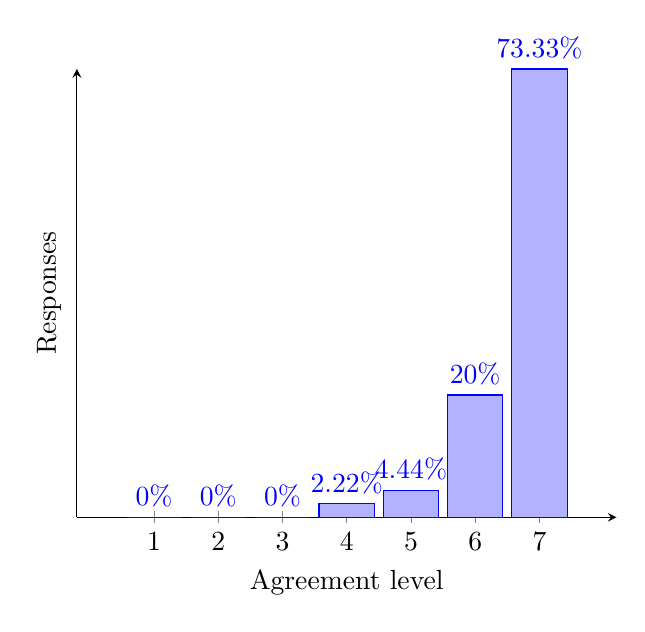
\begin{tikzpicture}
            \begin{axis}[
                ybar,
                xlabel={Agreement level},
                ylabel={Responses},
                ytick=\empty,
                xtick=data,
                axis x line=bottom,
                axis y line=left,
                enlarge x limits=0.2,
                bar width=20pt,
                nodes near coords={\pgfmathprintnumber\pgfplotspointmeta\%}
            ]
                \addplot coordinates {(1,0) (2,0) (3,0) (4,2.22) (5,4.44) (6,20) (7,73.33)};
            \end{axis}
        \end{tikzpicture}
        \caption{Responses to the question: "Privacy is important to me". Do you agree with this statement?}
        \label{fig:privacy_is_important_to_me}
    \end{center}
\end{figure}

\begin{figure}
    \begin{center}
        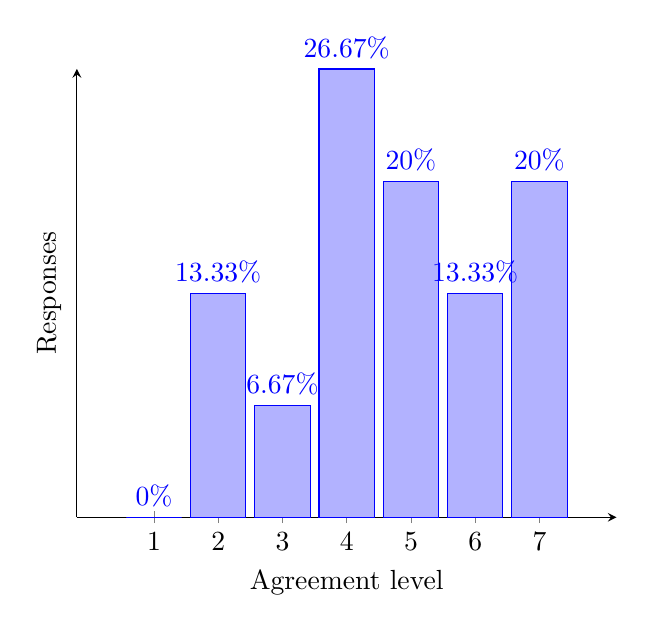
\begin{tikzpicture}
            \begin{axis}[
                ybar,
                xlabel={Agreement level},
                ylabel={Responses},
                ytick=\empty,
                xtick=data,
                axis x line=bottom,
                axis y line=left,
                enlarge x limits=0.2,
                bar width=20pt,
                nodes near coords={\pgfmathprintnumber\pgfplotspointmeta\%}
            ]
                \addplot coordinates {(1,0) (2,13.33) (3,6.67) (4,26.67) (5,20) (6,13.33) (7,20)};
            \end{axis}
        \end{tikzpicture}
        \caption{Responses to the question: "I know techniques to guarantee privacy and the protection of my data when I use the Internet". Do you agree with this statement?}
        \label{fig:techniques_to_guarantee_privacy}
    \end{center}
\end{figure}

\begin{figure}
    \begin{center}
        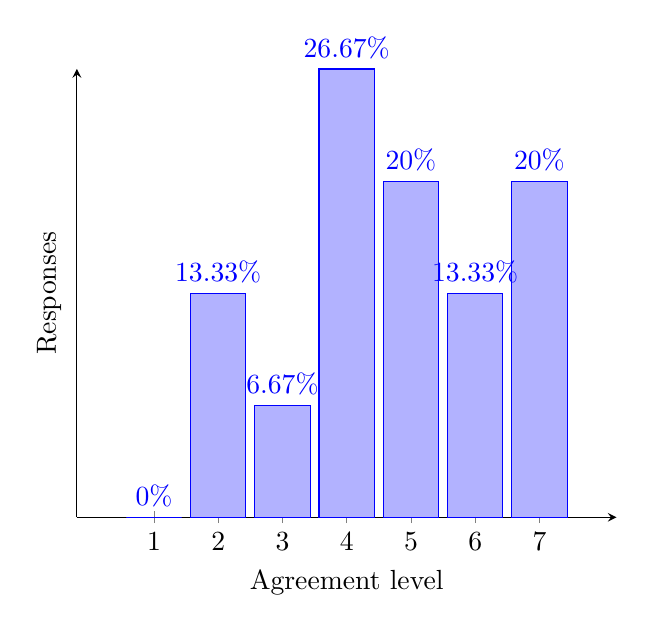
\begin{tikzpicture}
            \begin{axis}[
                ybar,
                xlabel={Agreement level},
                ylabel={Responses},
                ytick=\empty,
                xtick=data,
                axis x line=bottom,
                axis y line=left,
                enlarge x limits=0.2,
                bar width=20pt,
                nodes near coords={\pgfmathprintnumber\pgfplotspointmeta\%}
            ]
                \addplot coordinates {(1,0) (2,13.33) (3,6.67) (4,26.67) (5,20) (6,13.33) (7,20)};
            \end{axis}
        \end{tikzpicture}
        \caption{Responses to the question: Do you think your data privacy is important?}
        \label{fig:data_privacy_is_important}
    \end{center}
\end{figure}

\begin{figure}
    \begin{center}
        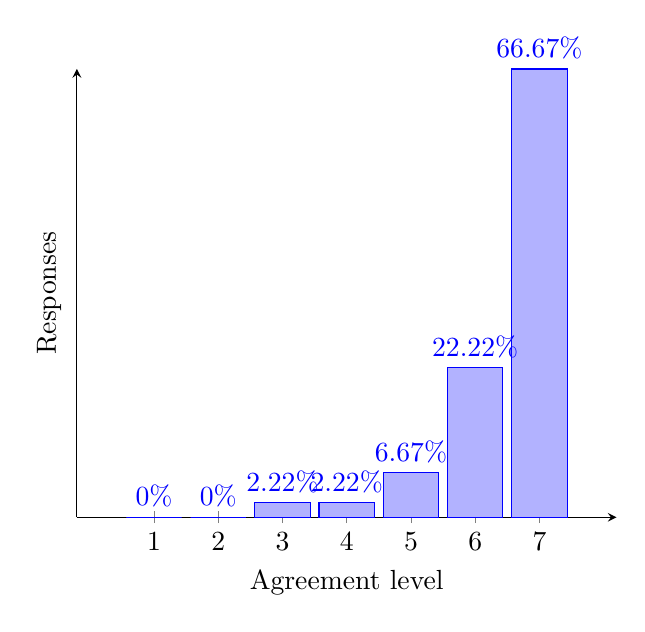
\begin{tikzpicture}
            \begin{axis}[
                ybar,
                xlabel={Agreement level},
                ylabel={Responses},
                ytick=\empty,
                xtick=data,
                axis x line=bottom,
                axis y line=left,
                enlarge x limits=0.2,
                bar width=20pt,
                nodes near coords={\pgfmathprintnumber\pgfplotspointmeta\%}
            ]
                \addplot coordinates {(1,0) (2,0) (3,2.22) (4,2.22) (5,6.67) (6,22.22) (7,66.67)};
            \end{axis}
        \end{tikzpicture}
        \caption{Responses to the question: Do you think your data privacy is important?}
        \label{fig:data_privacy_is_important}
    \end{center}
\end{figure}

\begin{figure}
    \begin{center}
        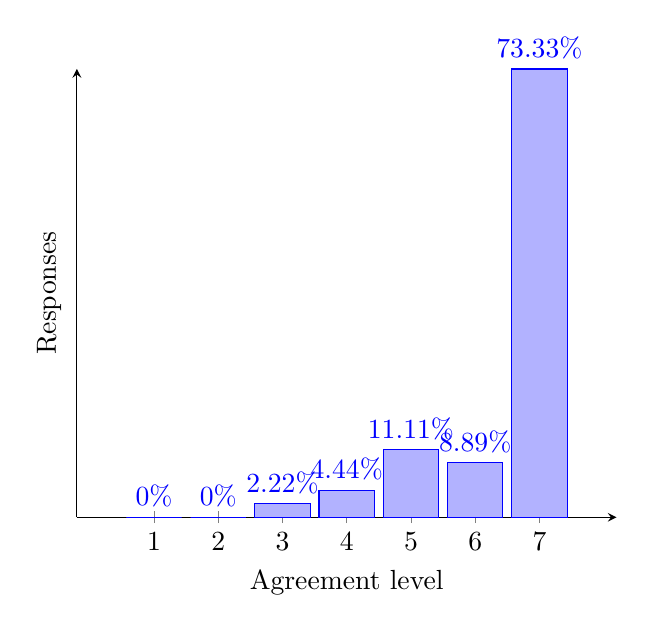
\begin{tikzpicture}
            \begin{axis}[
                ybar,
                xlabel={Agreement level},
                ylabel={Responses},
                ytick=\empty,
                xtick=data,
                axis x line=bottom,
                axis y line=left,
                enlarge x limits=0.2,
                bar width=20pt,
                nodes near coords={\pgfmathprintnumber\pgfplotspointmeta\%}
            ]
                \addplot coordinates {(1,0) (2,0) (3,2.22) (4,4.44) (5,11.11) (6,8.89) (7,73.33)};
            \end{axis}
        \end{tikzpicture}
        \caption{Responses to the question: Do you think your data privacy is relevant nowadays?}
        \label{fig:data_privacy_relevant}
    \end{center}
\end{figure}

\begin{figure}
    \centering
    \begin{tikzpicture}
        \pie{2.22/Do not know,
            2.22/Disagree,
            95.56/Agree}
    \end{tikzpicture}
    \caption{Responses to the question: "Data privacy is a human right". Do you agree with this statement?}
    \label{fig:privacy_human_right}
\end{figure}

\begin{figure}
    \centering
    \begin{tikzpicture}
        \pie{4.44/Do not know,
            0/Disagree,
            95.56/Agree}
    \end{tikzpicture}
    \caption{Responses to the question: "Data privacy is a consumer right". Do you agree with this statement?}
    \label{fig:privacy_consumer_right}
\end{figure}

\begin{figure}
    \centering
    \begin{tikzpicture}
        \pie[explode = 0.1]{46.67/No,
            53.33/Yes}
    \end{tikzpicture}
    \caption{Responses to the question: In your opinion, are security and privacy synonymous?}
    \label{fig:security_equals_privacy}
\end{figure}

\begin{figure}
    \begin{center}
        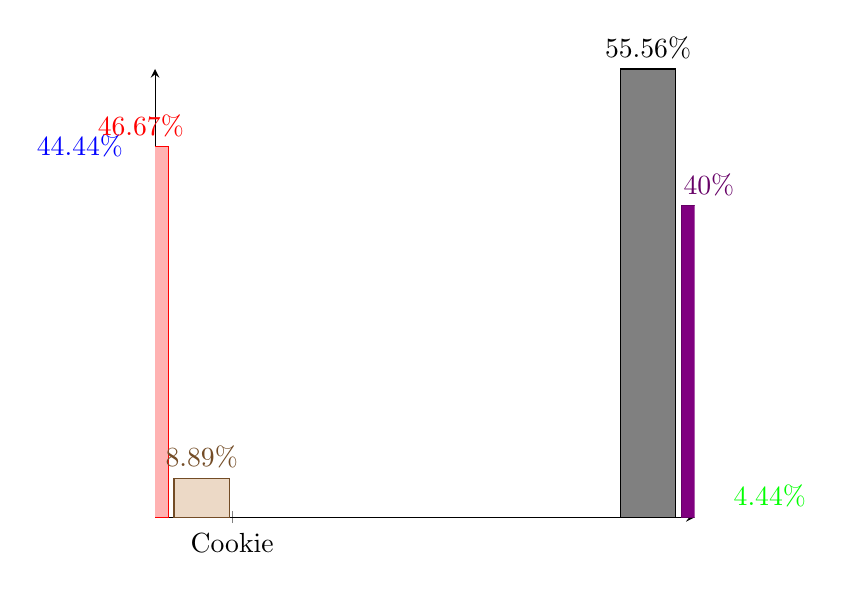
\begin{tikzpicture}
            \begin{axis}[
                symbolic x coords={Cookie, Wireless networks},
                ybar,
                ytick=\empty,
                xtick=data,
                axis x line=bottom,
                axis y line=left,
                enlarge x limits=0.2,
                bar width=20pt,
                nodes near coords={\pgfmathprintnumber\pgfplotspointmeta\%}
            ]
                \addplot coordinates {(Cookie,44.44)};
                \addplot coordinates {(Cookie,46.67)};
                \addplot coordinates {(Cookie,8.89)};
                \addplot coordinates {(Wireless networks,55.56)};
                \addplot coordinates {(Wireless networks,40)};
                \addplot coordinates {(Wireless networks,4.44)};
            \end{axis}
        \end{tikzpicture}
        \caption{Responses to the question: How familiar are you with the following terms?}
        \label{fig:familiar_terms}
    \end{center}
\end{figure}

\begin{figure}
    \begin{center}
        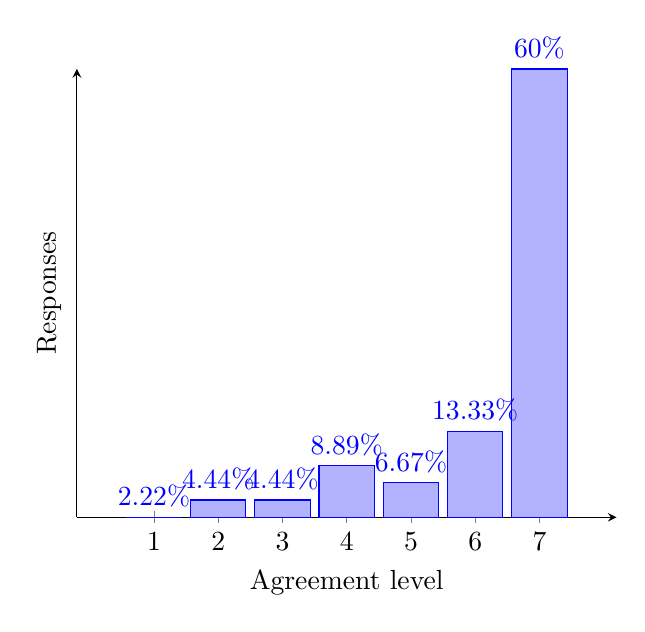
\begin{tikzpicture}
            \begin{axis}[
                ybar,
                xlabel={Agreement level},
                ylabel={Responses},
                ytick=\empty,
                xtick=data,
                axis x line=bottom,
                axis y line=left,
                enlarge x limits=0.2,
                bar width=20pt,
                nodes near coords={\pgfmathprintnumber\pgfplotspointmeta\%}
            ]
                \addplot coordinates {(1,2.22) (2,4.44) (3,4.44) (4,8.89) (5,6.67) (6,13.33) (7,60)};
            \end{axis}
        \end{tikzpicture}
        \caption{Responses to the question: During your day-to-day life, how often do you use your phone to access the internet?}
        \label{fig:phone_access_internet}
    \end{center}
\end{figure}

\begin{figure}
    \begin{center}
        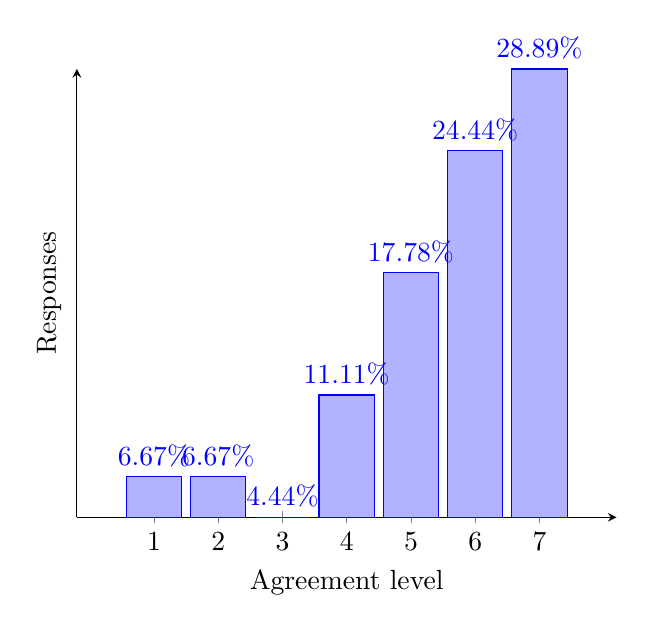
\begin{tikzpicture}
            \begin{axis}[
                ybar,
                xlabel={Agreement level},
                ylabel={Responses},
                ytick=\empty,
                xtick=data,
                axis x line=bottom,
                axis y line=left,
                enlarge x limits=0.2,
                bar width=20pt,
                nodes near coords={\pgfmathprintnumber\pgfplotspointmeta\%}
            ]
                \addplot coordinates {(1,6.67) (2,6.67) (3,4.44) (4,11.11) (5,17.78) (6,24.44) (7,28.89)};
            \end{axis}
        \end{tikzpicture}
        \caption{Responses to the question: "I am concerned about my privacy when using my mobile phone when accessing the internet". Do you agree with this statement?}
        \label{fig:concerned_privacy_using_phone}
    \end{center}
\end{figure}

\begin{figure}
    \begin{center}
        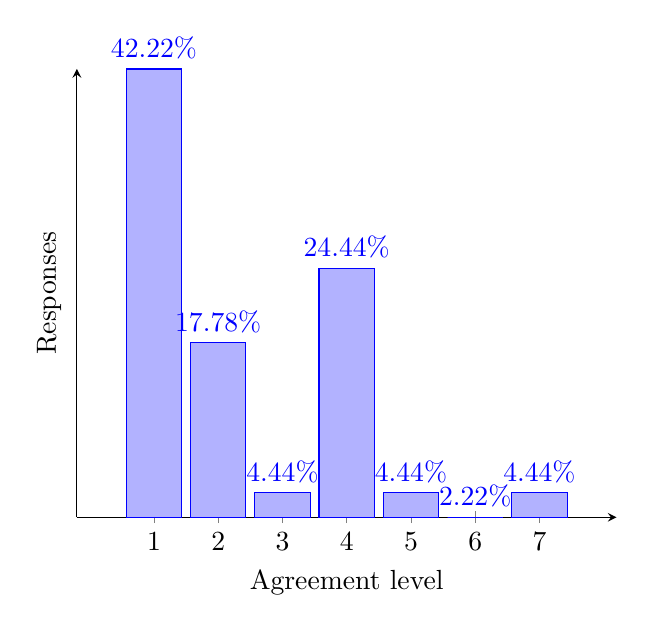
\begin{tikzpicture}
            \begin{axis}[
                ybar,
                xlabel={Agreement level},
                ylabel={Responses},
                ytick=\empty,
                xtick=data,
                axis x line=bottom,
                axis y line=left,
                enlarge x limits=0.2,
                bar width=20pt,
                nodes near coords={\pgfmathprintnumber\pgfplotspointmeta\%}
            ]
                \addplot coordinates {(1,42.22) (2,17.78) (3,4.44) (4,24.44) (5,4.44) (6,2.22) (7,4.44)};
            \end{axis}
        \end{tikzpicture}
        \caption{Responses to the question: "I consider that accessing the internet through my phone is safer than through a computer". Do you agree with this statement?}
        \label{fig:phone_safer_than_computer}
    \end{center}
\end{figure}

\begin{figure}
    \begin{center}
        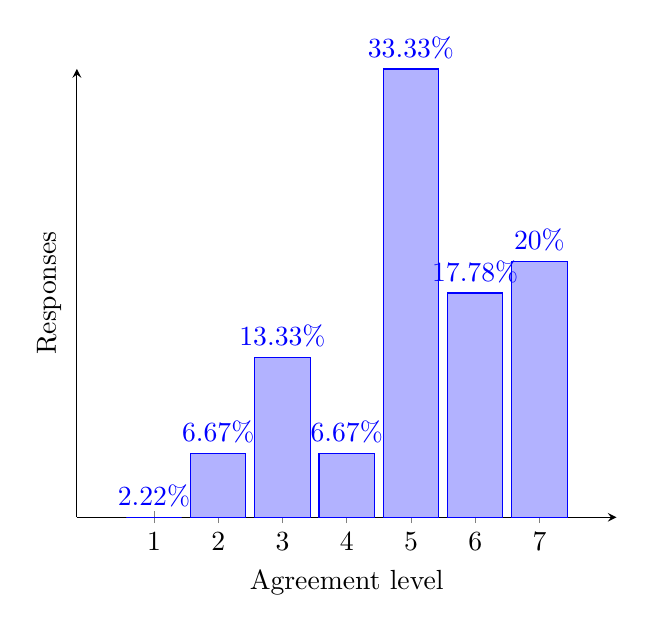
\begin{tikzpicture}
            \begin{axis}[
                ybar,
                xlabel={Agreement level},
                ylabel={Responses},
                ytick=\empty,
                xtick=data,
                axis x line=bottom,
                axis y line=left,
                enlarge x limits=0.2,
                bar width=20pt,
                nodes near coords={\pgfmathprintnumber\pgfplotspointmeta\%}
            ]
                \addplot coordinates {(1,2.22) (2,6.67) (3,13.33) (4,6.67) (5,33.33) (6,17.78) (7,20)};
            \end{axis}
        \end{tikzpicture}
        \caption{Responses to the question: "I try to block the collection of data from applications installed on my phone". Do you agree with this statement?}
        \label{fig:block_collection_data_applications}
    \end{center}
\end{figure}

\begin{figure}
    \begin{center}
        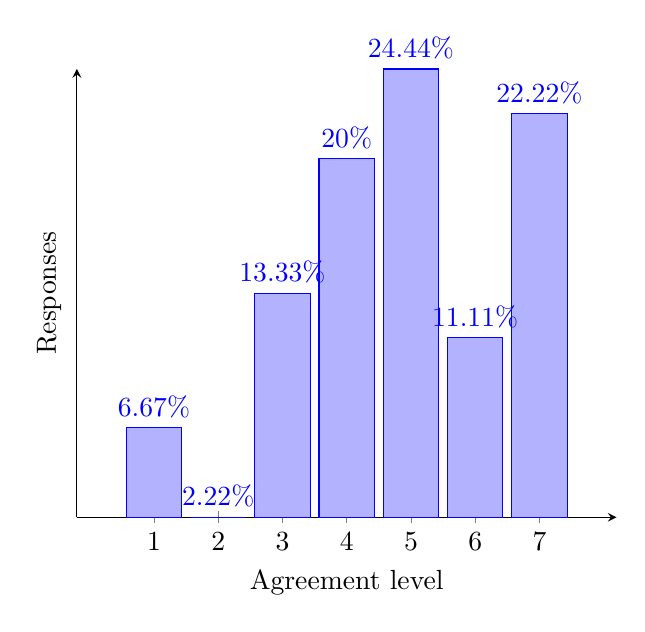
\begin{tikzpicture}
            \begin{axis}[
                ybar,
                xlabel={Agreement level},
                ylabel={Responses},
                ytick=\empty,
                xtick=data,
                axis x line=bottom,
                axis y line=left,
                enlarge x limits=0.2,
                bar width=20pt,
                nodes near coords={\pgfmathprintnumber\pgfplotspointmeta\%}
            ]
                \addplot coordinates {(1,6.67) (2,2.22) (3,13.33) (4,20) (5,24.44) (6,11.11) (7,22.22)};
            \end{axis}
        \end{tikzpicture}
        \caption{Responses to the question: How often do you allow the use of cookies?}
        \label{fig:allow_cookies}
    \end{center}
\end{figure}

\begin{figure}
    \centering
    \begin{tikzpicture}
        \pie[explode = 0.1]{48.89/No,
            51.11/Yes}
    \end{tikzpicture}
    \caption{Responses to the question: Are you aware of the concept of "profiling" or "automated processing of personal information"?}
    \label{fig:aware_profiling}
\end{figure}

\begin{figure}
    \centering
    \begin{tikzpicture}
        \pie[explode = 0.1]{33.33/I do not know,
            8.89/No,
            57.78/Yes}
    \end{tikzpicture}
    \caption{Responses to the question: Do you consider that your internet activity contributes to the development of profiling?}
    \label{fig:activity_contributes_profiling}
\end{figure}

\subsection{Stage 2: Study in Context, an Application}

This work proposes an application that gives users information about IoT
devices that inhabit their surroundings, like the type of information these devices
collect and what privacy options are available. This application is developed
for mobile phones due to the fact that these are the most used devices
and people take them everywhere they go, this is important because the application
uses georeferencing to show the location of the IoT devices. This application
has two main objectives, the first is to inform and educate users in order improve
their digital literacy on this particular field (privacy on IoT systems, and
IoT in general) and the other being to give users a way to make informed decisions
to protect their private data, in a concise and convenient place. Generally
the application will show the geolocation of the IoT devices, what type of
device it is, what type of data is being collect by the device. The application
will not detect the devices by itself, this will be done by the users themselves,
in the first iterations of the application it was discussed that the application
itself would automatically detect the devices by using some kind of sniffer
and would categorize what type of device it was and what type of data it
was collecting but it was discovered that this approach was too complex and
so it was not feasible to do with the constraints of this thesis. The application
is developed with Flutter, other options considered were React Native or a
progressive web application, but Flutter uses ahead of time and just in time
compilation, with Dart as it is programming language, while React Native uses
the Javascript programming language that was never created for mobile programming,
so it uses a bridge to convert Javascript to native components for Android
or iOS. Flutter has better performance and as such it was the chosen framework
for this application.

The first step before creating any prototypes or starting the development was
creating a software requirements specification, as can be read on appendix \ref{appendix:a},
delineating the scope and vision for the application; the involved stakeholders;
containing contextual, data-flow and swimlane diagrams; software requirements, including
business, technology, functional and non-functional requirements; use cases
and requirements prioritisation.

Users can, when they start the application for the first time, freely use it to see
which devices are in their vicinity,
information about the devices, information about the application itself, and
information about privacy in general and more specifically privacy in IoT systems
which they can use to improve their digital literacy. What they cannot do is
add a new device to the application or edit a device's information. The user has
to create an account first to do these operations. The decision to add an
account creation before the user can add or edit a device is to prevent
bad actors to add bogus data to the application making unusable for the majority
of people, this solution doesn't completely solve this issue (because bad actors
can still create an account and add bogus data anyway) but it helps to slow
down the insertion of bad data.

Upon account creation the only data entry that can be considered sensitive that
the user has to input is an email address.
After the user has created an account and logs in, the user can add devices to the application with the following information:

\begin{itemize}
    \item[$\bullet$]
    The \textbf{name of the device}: This serves to differenciate between the various devices on the application and as such should be unique to each device, it is used on various routes and is one of the first fields that users see about a device. A single device doen't have an \textit{official} name, what is more probable is that the device has a model name or is part of a system with it's own name. The user creates the name, this could be abused by bad actors but it is extremelly discouraged. It is used for asthethic reasons.
    \item[$\bullet$]
    The \textbf{category of the device}: This is used to categorize each devices main type of information that the device is collecting. These can be of the following:
    \begin{itemize}
        \item[$\circ$] \textbf{Visual}: The device mainly collects visual information with maybe a video camera.
        \item[$\circ$] \textbf{Audio}: The device mainly collects audio information with a microphone.
        \item[$\circ$] \textbf{Presence}: The device can detect the presence of nearby objects or persons. This is not the same as the location category because the device does not know the location of an individual, it merely knows that the individual is nearby. These type of devices can be used, for example, to collect information about how many people frequent a specific store.
        \item[$\circ$] \textbf{Location}: The device can detect the exact or approximate location of an individual, it can use GPS to get this kind of information.
        \item[$\circ$] \textbf{Biometrics}: The devices collects biometric data, this can be the number of steps an individual (or animal) takes, or health related data like the heart beat.
        \item[$\circ$] \textbf{Environment}: These type of devices collect environmental data, they can be used for aggriculture or weather forecasting by collecting, for example, temperature, humidity or wind speed/direction data.
        \item[$\circ$] \textbf{Unique identification}: This category is for a device that can uniquely identify an individual, the device itself most likely is not capable of doing it but with other information that the device has access to, it can be used to cross reference of information and as such uniquely identify a person. An example of this would be a device a device that can collect visual data and with facial recognition used against other data in a database it can uniquely identify an individual.
    \end{itemize}
    \item[$\bullet$]
    The \textbf{purpose for the data collection}: Defines what is the purpose for the collection of the data, if a device collects temperature and humidity data and is used by a weather based company or government agency then the purpose for the data collection is for weather forecasting.
    \item[$\bullet$]
    \textbf{Who has access to the collected data}: Disclose an individual or group of individuals that have access to the data of the device, if the device is part of a closed system it can be that only an individual as access to the data but most likely various groups of people have access to the data, some with more data than others depending on the permissions they have. If the device publicizes its data then everyone has access to it.
    \item[$\bullet$]
    \textbf{For how long is the data stored}: Pinpoint the duration of the stored data in the device or system, due to legislation passed in various countries this duration has a limit, in some cases the data cannot be stored for more than one year.
    \item[$\bullet$]
    \textbf{Can the data identify anyone}: Used to quickly identify if a partitular device can identify an idividual or not. If the device belongs to the "Unique identification" category then this should be active.
    \item[$\bullet$]
    \textbf{What is being done with the data}: This could be assumed to be similar to the \textbf{purpose} field mentioned above but it should be used to diagnose what is being done now with the data collected, in certain situations it might coincide with the purpose for the data collection.
    \item[$\bullet$]
    \textbf{Privacy options}: The user can insert an url for the device's privacy options, in some cases the device, or company, has a website with information on privacy options, or privacy policy. If the device uses a mobile application then a link to the this application can be inserted here.
    \item[$\bullet$]
    \textbf{Coordinates of the device}: Used to express the lagitude and longitude of the device so that it can be shown on the map, on the homepage of the application.
    \item[$\bullet$]
    \textbf{Who owns the device}: Who is the device owner, if it belongs to an organization then the name of the organization should appear here otherwise if the device belongs to a person then the person's name should \textbf{not} appear, it should say private or something similar.
\end{itemize}

The user is not required to provide information to satisfy all items on this list, the
only information that is required in order to add a device to the application is
the name, category and coordinates of the device, all other
information is optional but should be provided for the sake of guaranting a good
experience to other users of the application. The information provided
should be verified by the user beforehand so that bogus data does not clutter
the application, in this case there are no absolute ways of guaranting this
but the maintainer of the application edit wrong information or in some
cases remove it, other users can also edit any device data. This is an
open platform so it is expected that users act in good faith.

One problem this application faces, and other applications where there is
some kind of user interaction also face, is the fact that some bad
actors will abuse the system by creating many fake accounts, by
data scrapping, by adding bogus data or by replacing existing information
with bogus data.

% Types of data:
% Health
% Visual
% Audio
% Presence (if user is nearby)
% Location (precise location of user)
% Biometrics
% Environment
% Unique identification (with the help of other means)

% Infomation to be added to the app:
% What is the purpose of the data collection
% Who can access the data
% For how long is it stored
% Can the data identify anyone
% What is done with this data

% \section{Current Stage of the Work}

% The preliminary results of the study, based on 10 responses, show that everyone
% agrees that privacy is important to them and some people know that they
% should not share their personal information with anyone they do not trust
% (like clicking on random urls or using unprotected websites/software), but
% most of them think that privacy and security are the same concept, most
% respondents also do not read privacy notices but accept them to access the
% information they want to get to, most respondents use their devices mostly
% to access social networks and for work, when it comes to IoT, there is a
% dissonance between knowing the term and using devices like smart watches
% or RFID enabled devices, from the respondents that answered yes to using
% IoT devices most use because of work. It is also noted that most respondent
% have a background in engineering, so the responses are skewed. As a result,
% the survey will remain open to gather a larger number of responses and participants
% for more significant results and generalizations.

% \begin{table}[ht]
% \centering
% \begin{adjustbox}{width=0.5\textwidth}
% \small
% \noindent\begin{tabular}{p{0.17\textwidth}*{20}{|p{0.01\textwidth}}|}
% \hline
% \multicolumn{0}{|c|}{Work plan}
%     & \multicolumn{4}{c|}{January}
%     & \multicolumn{4}{c|}{February}
%     & \multicolumn{4}{c|}{March}
%     & \multicolumn{4}{c|}{April}
%     & \multicolumn{4}{c|}{May}
%     \\
% \hline
% \hline
% \multicolumn{0}{|l|}{Week}
%     & 1 & 2 & 3 & 4 & 1 & 2 & 3 & 4& 1 & 2 & 3 & 4& 1 & 2 & 3 & 4& 1 & 2 & 3 & 4 \\
% \hline
% % using the on macro to fill in twenty cells as `on'
% \multicolumn{0}{|l|}{Discovery and planning}
%     & \cellcolor[cmyk]{1,1,0,0}&&&& &&&& &&&& &&&&&&& \\
% \hline
% \multicolumn{0}{|l|}{Research enquiry}
%     & \cellcolor[cmyk]{1,1,0,0} & \cellcolor[cmyk]{1,1,0,0} & \cellcolor[cmyk]{1,1,0,0} & \cellcolor[cmyk]{1,1,0,0} & \cellcolor[cmyk]{1,1,0,0} & \cellcolor[cmyk]{1,1,0,0} & \cellcolor[cmyk]{1,1,0,0} & \cellcolor[cmyk]{1,1,0,0} & \cellcolor[cmyk]{1,1,0,0} & \cellcolor[cmyk]{1,1,0,0} & \cellcolor[cmyk]{1,1,0,0} & \cellcolor[cmyk]{1,1,0,0} &&&& &&&& \\
% \hline
% \multicolumn{0}{|l|}{State of the art}
%     & \cellcolor[cmyk]{1,1,0,0} & \cellcolor[cmyk]{1,1,0,0} & \cellcolor[cmyk]{1,1,0,0} & \cellcolor[cmyk]{1,1,0,0} & \cellcolor[cmyk]{1,1,0,0} & \cellcolor[cmyk]{1,1,0,0} & \cellcolor[cmyk]{1,1,0,0} & \cellcolor[cmyk]{1,1,0,0} &&&& &&&& &&&& \\
% \hline
% \multicolumn{0}{|l|}{Project requirements}
%     & \cellcolor[cmyk]{1,1,0,0} & \cellcolor[cmyk]{1,1,0,0} & \cellcolor[cmyk]{1,1,0,0} & \cellcolor[cmyk]{1,1,0,0} &&&& &&&& &&&& &&&& \\
% \hline
% \multicolumn{0}{|l|}{Wireframes and user stories}
%     &&&& & \cellcolor[cmyk]{1,1,0,0} & \cellcolor[cmyk]{1,1,0,0} & \cellcolor[cmyk]{1,1,0,0} & \cellcolor[cmyk]{1,1,0,0} &&&& &&&& &&&& \\
% \hline
% \multicolumn{0}{|l|}{Prototyping and refinement}
%     &&&&&& && \cellcolor[cmyk]{1,1,0,0} & \cellcolor[cmyk]{1,1,0,0} & \cellcolor[cmyk]{1,1,0,0} & \cellcolor[cmyk]{1,1,0,0} &&&& &&&& &  \\
% \hline
% \multicolumn{0}{|l|}{Development}
%     &&&& &&&& & \cellcolor[cmyk]{1,1,0,0} & \cellcolor[cmyk]{1,1,0,0} & \cellcolor[cmyk]{1,1,0,0} & \cellcolor[cmyk]{1,1,0,0} & \cellcolor[cmyk]{1,1,0,0} & \cellcolor[cmyk]{1,1,0,0} & \cellcolor[cmyk]{1,1,0,0} & \cellcolor[cmyk]{1,1,0,0} & \cellcolor[cmyk]{1,1,0,0} & \cellcolor[cmyk]{1,1,0,0} & \cellcolor[cmyk]{1,1,0,0} & \cellcolor[cmyk]{1,1,0,0} \\
% \hline
% \multicolumn{0}{|l|}{Tests and iterations}
%     &&&& &&&& &&& & \cellcolor[cmyk]{1,1,0,0} & \cellcolor[cmyk]{1,1,0,0} & \cellcolor[cmyk]{1,1,0,0} & \cellcolor[cmyk]{1,1,0,0} & \cellcolor[cmyk]{1,1,0,0} &&&&  \\
% \hline
% \multicolumn{0}{|l|}{Release and documentation}
%     &&&& &&&& &&&& &&&& & \cellcolor[cmyk]{1,1,0,0} & \cellcolor[cmyk]{1,1,0,0} & \cellcolor[cmyk]{1,1,0,0} & \cellcolor[cmyk]{1,1,0,0} \\
% \hline
% \end{tabular}
% \end{adjustbox}
% \vspace{1em}
% \caption{Work plan timeline}
% \label{workchart}
% \end{table}

% As can be seen in Table \ref{workchart}, the first months will involve the
% design of the application and the enquiry of the study followed by the development
% of the application and the synthesis of the study, and finally testing and
% refinement of the application. Because of the exploratory nature of this
% work the application might suffer alterations to the design, specially in
% the testing stage, and also depending on the results of the study.

\begin{figure}
    \centering
    \begin{subfigure}{0.33\textwidth}
        \centering
        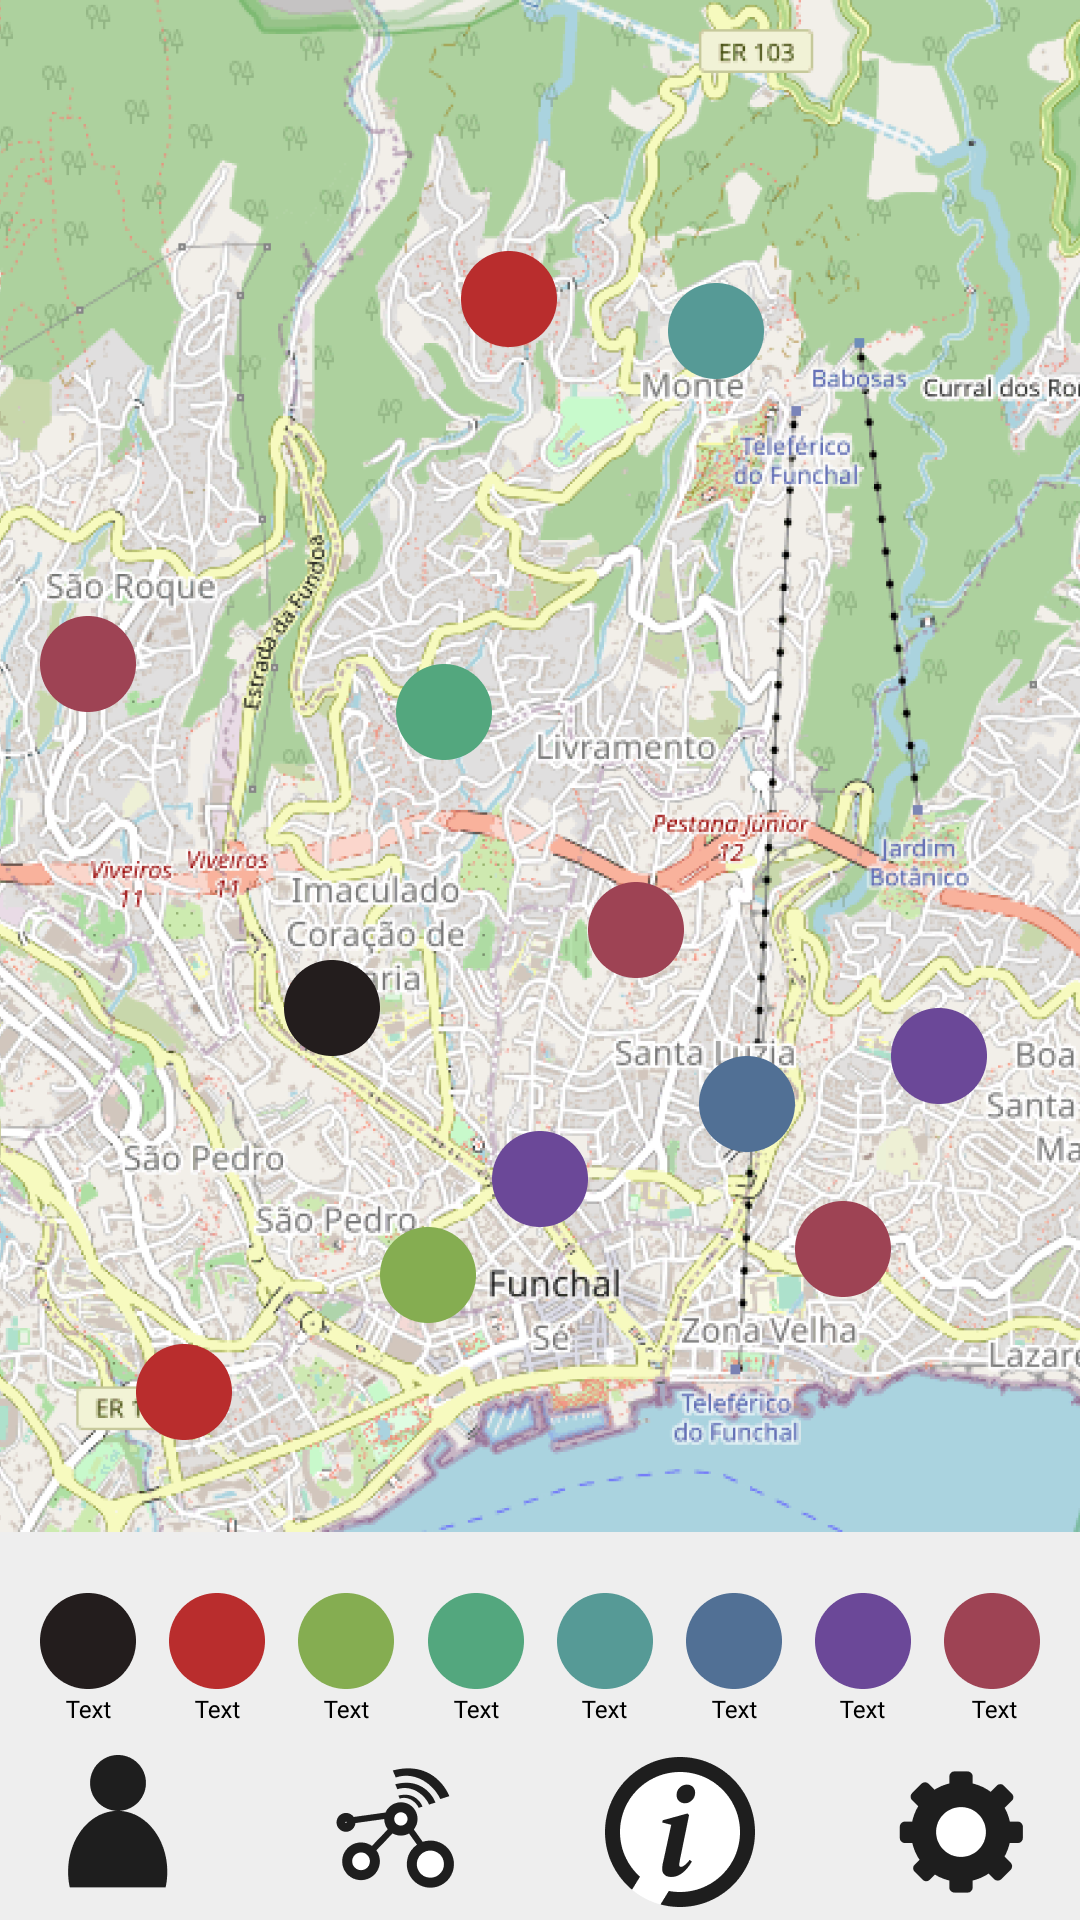
\includegraphics[width=130pt]{../assets/images/low_homepage.png}
        \caption{}
        \label{fig:home}
    \end{subfigure}%
    \begin{subfigure}{0.33\textwidth}
        \centering
        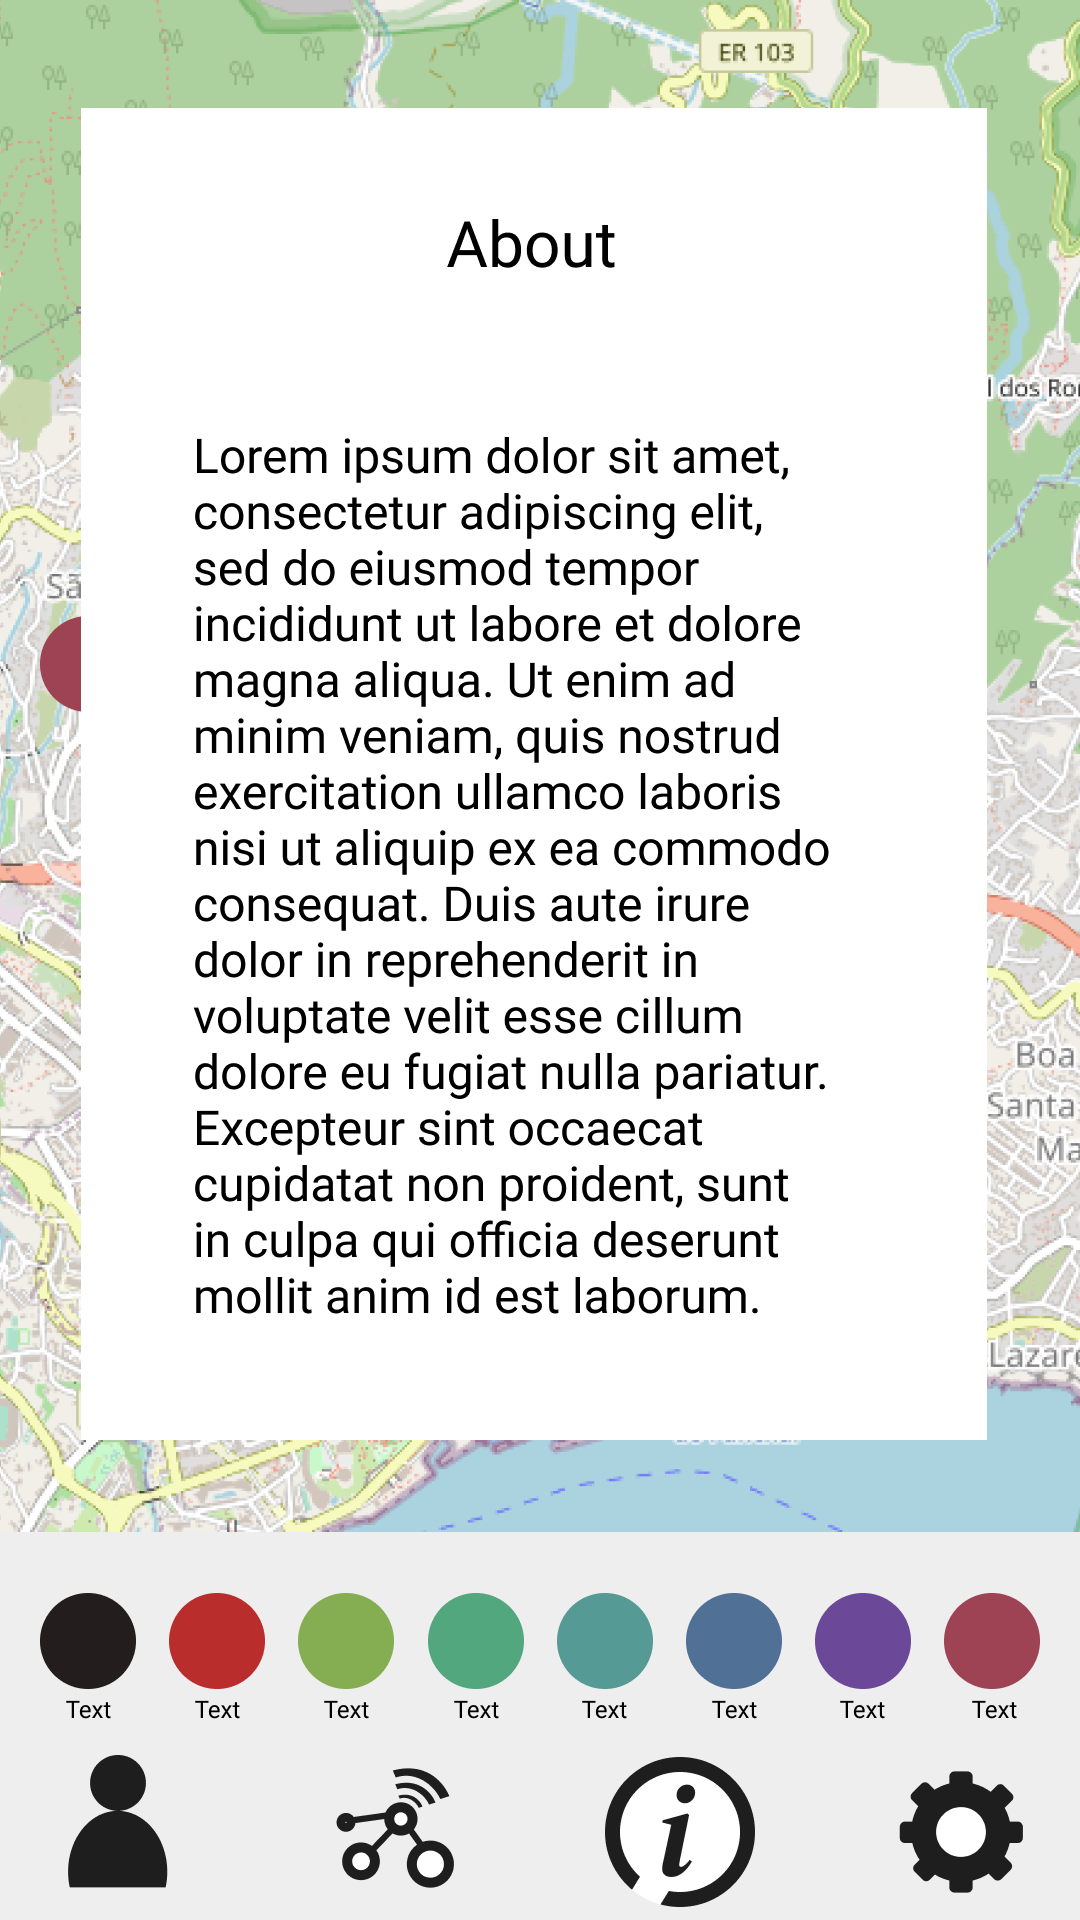
\includegraphics[width=130pt]{../assets/images/low_about.png}
        \caption{}
        \label{fig:about}
    \end{subfigure}%
    \begin{subfigure}{0.33\textwidth}
        \centering
        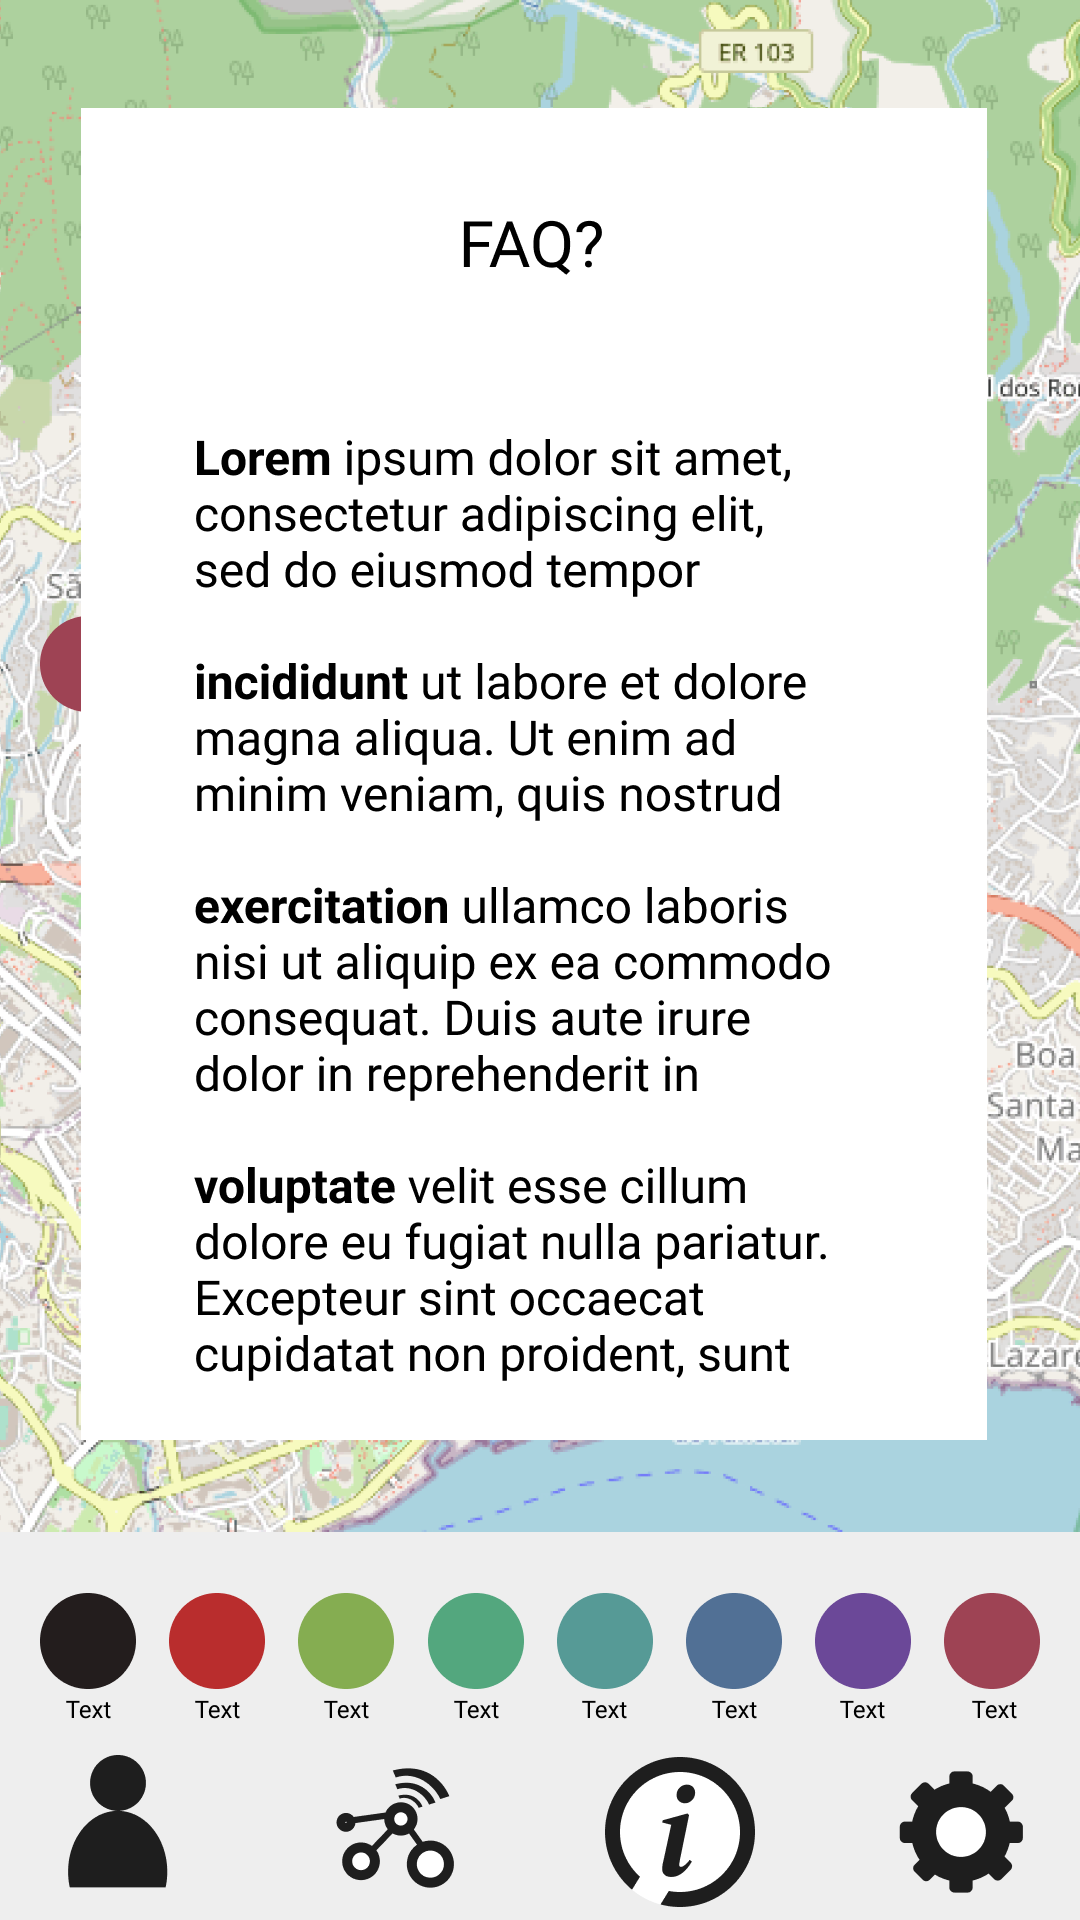
\includegraphics[width=130pt]{../assets/images/low_more_info.png}
        \caption{}
        \label{fig:faq}
    \end{subfigure}%
    \caption{Low level prototype of (a) homepage, (b) about and (c) FAQ pages.}
    \label{fig:lowlevelprototype}
\end{figure}

After creating the software requirements specification, the prototypes were
created. For the creation of the prototypes the following tools were used: Figma
and GIMP.

At first a low level prototype was made in order to understand the
general design and user interaction of the application. Figure \ref{fig:lowlevelprototype}
shows tree pages of the low level prototype, these are the homepage, about
and faq pages, this prototype has a navigation menu on the bottom where the
other pages of the application can be selected along with some information
above the page icons, this information is supposed to be the categories of
the devices, the logic would be that the user could tap one of these categories
and only devices of the category should be displayed on the map. It can
be seen that between the three pages the map stays in the background and
the various pages work like an overlay on the homepage, this would be
changed in subsequent prototype versions.

\begin{figure}
    \centering
    \begin{subfigure}{0.33\textwidth}
        \centering
        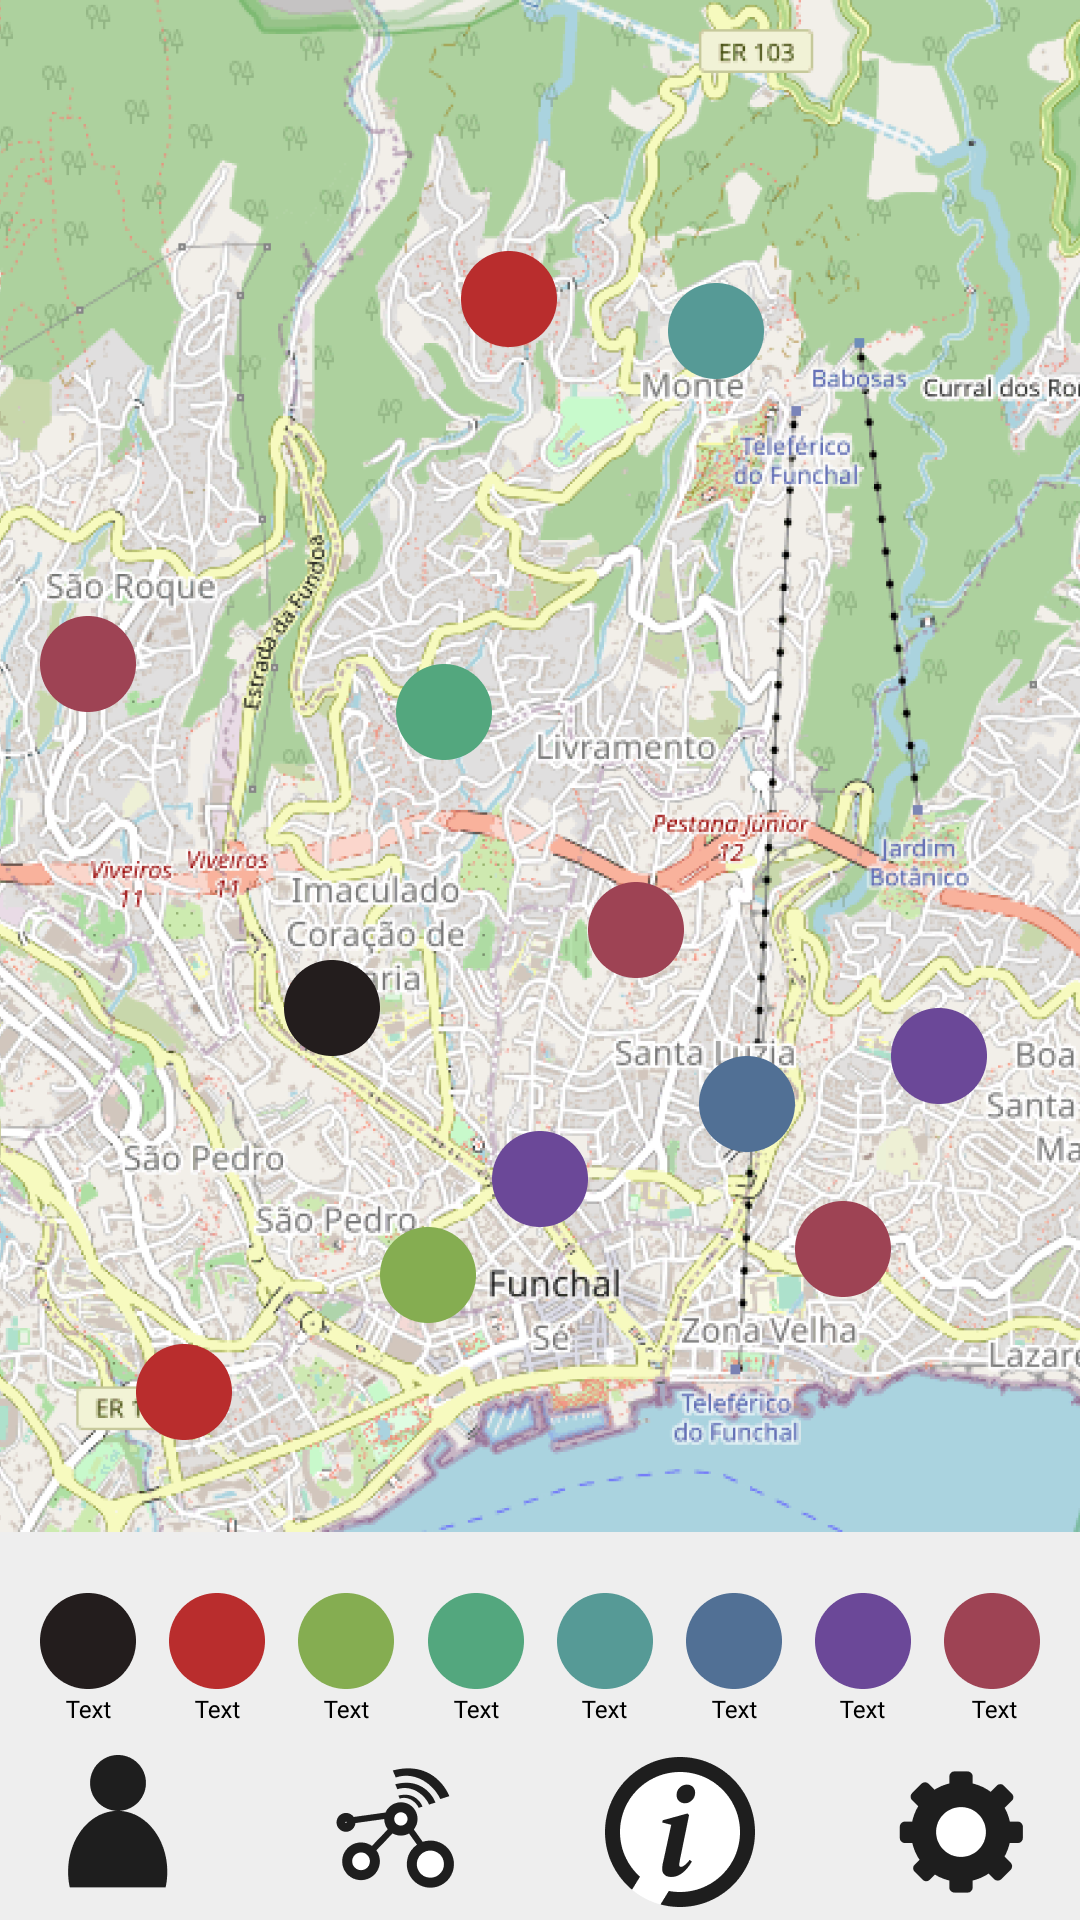
\includegraphics[width=130pt]{../assets/images/low_homepage.png}
        \caption{}
        \label{fig:home}
    \end{subfigure}%
    \begin{subfigure}{0.33\textwidth}
        \centering
        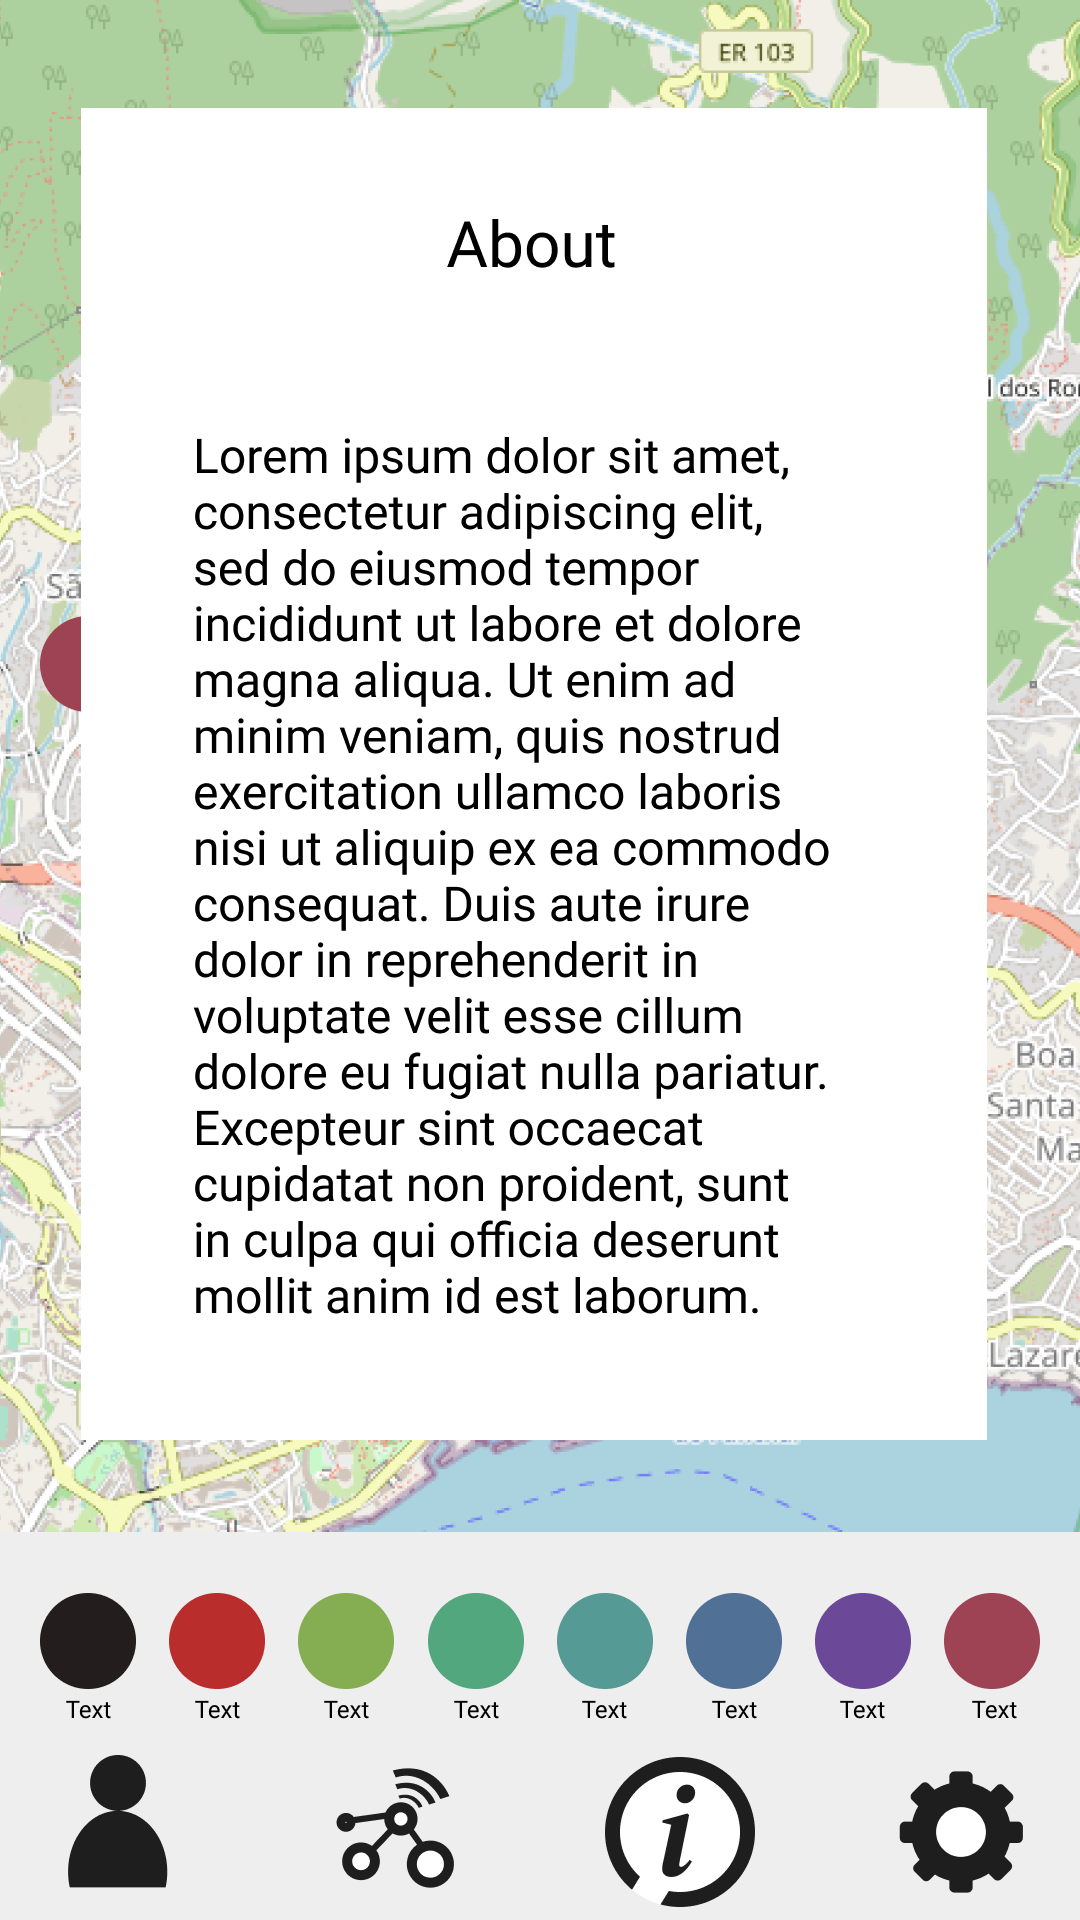
\includegraphics[width=130pt]{../assets/images/low_about.png}
        \caption{}
        \label{fig:about}
    \end{subfigure}%
    \begin{subfigure}{0.33\textwidth}
        \centering
        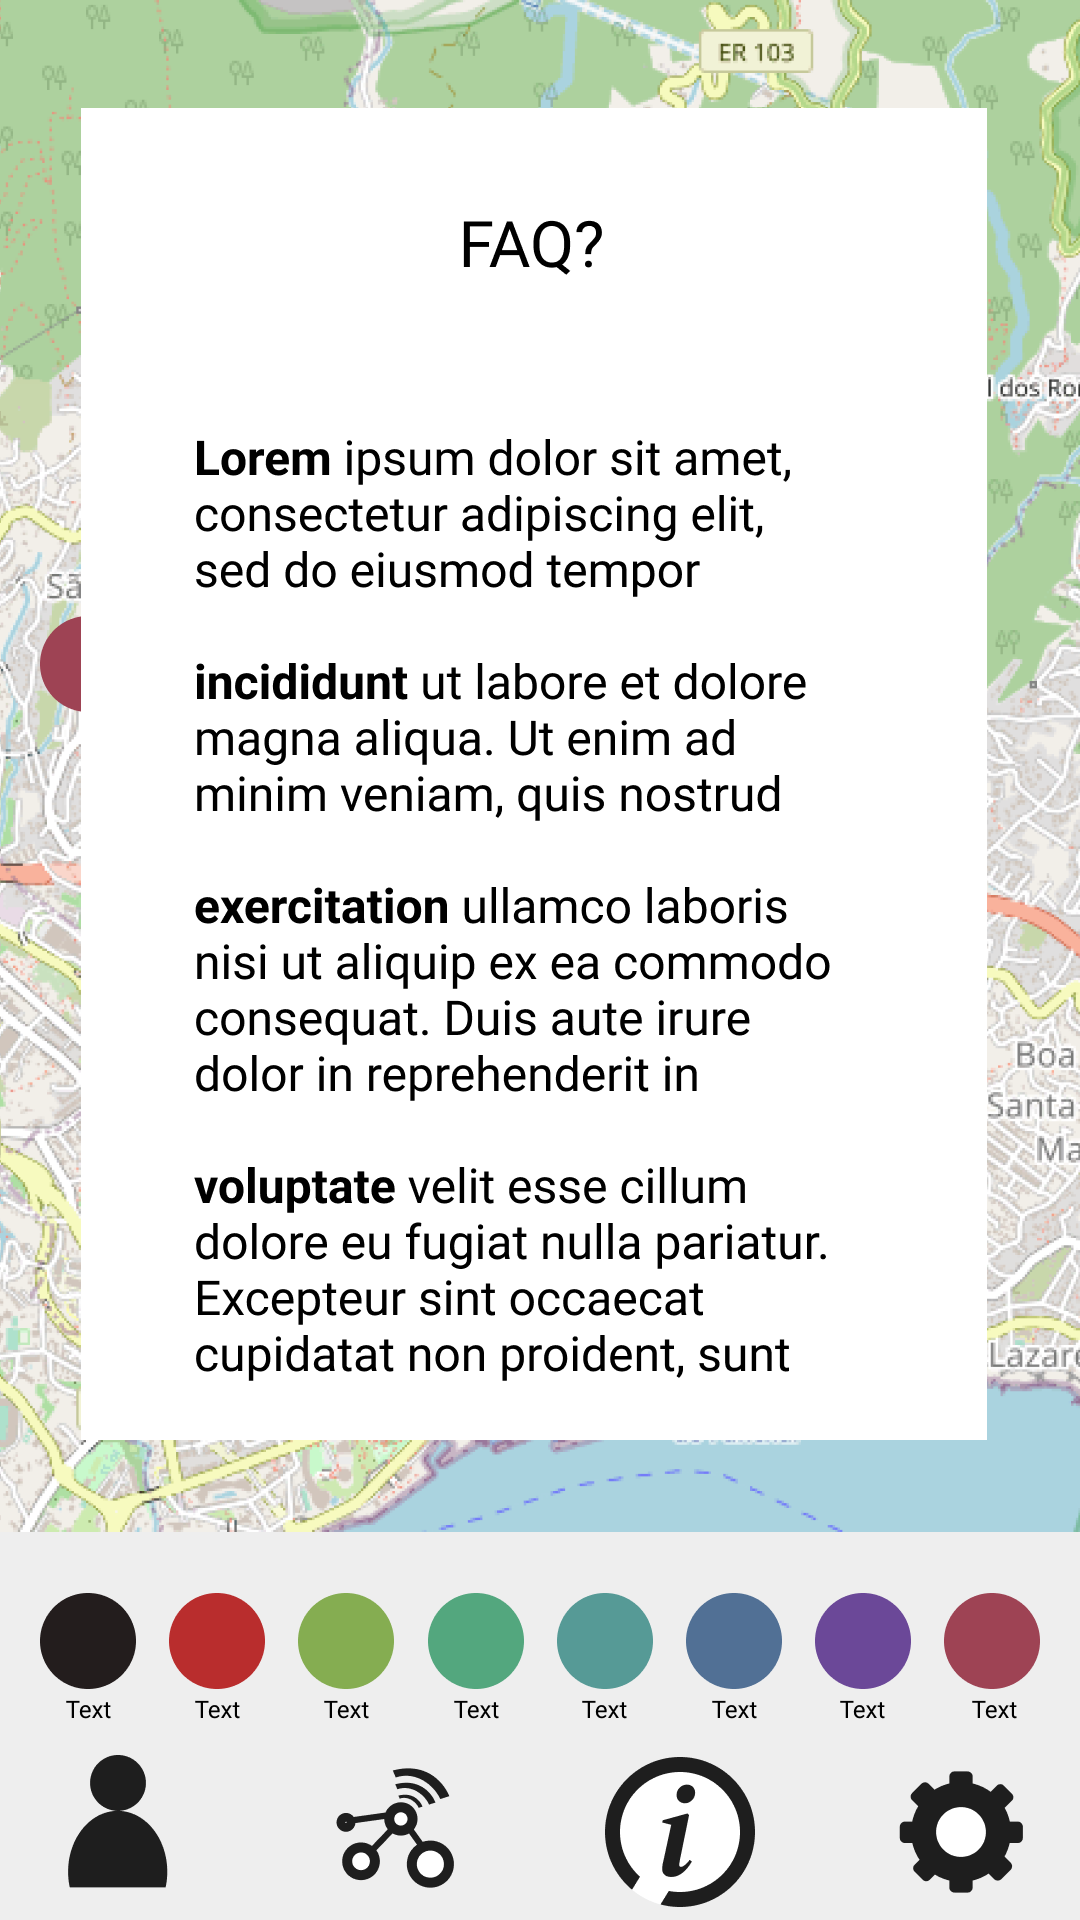
\includegraphics[width=130pt]{../assets/images/low_more_info.png}
        \caption{}
        \label{fig:faq}
    \end{subfigure}%
    \caption{Medium level prototype of (a) homepage, (b) about and (c) FAQ pages.}
    \label{fig:mediumlevelprototype}
\end{figure}

\begin{figure}
    \centering
    \begin{subfigure}{0.33\textwidth}
        \centering
        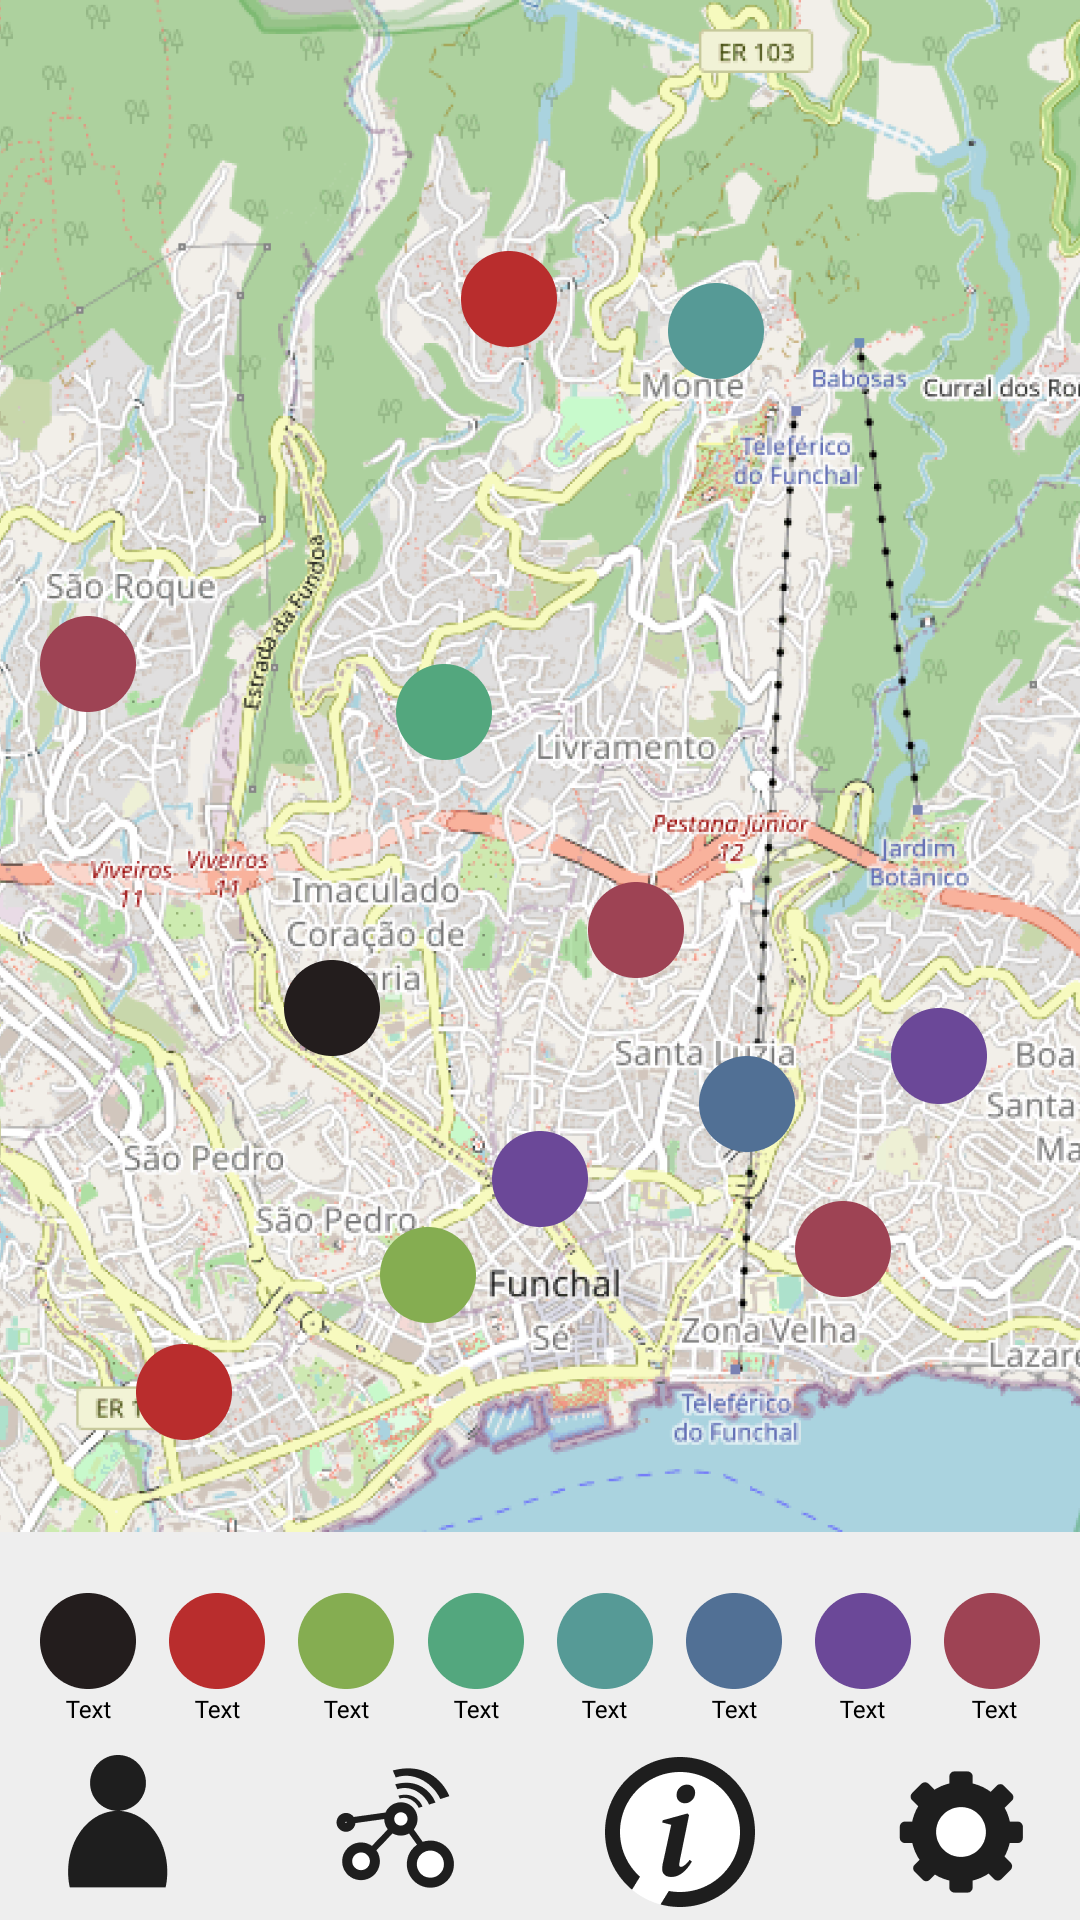
\includegraphics[width=130pt]{../assets/images/low_homepage.png}
        \caption{}
        \label{fig:home}
    \end{subfigure}%
    \begin{subfigure}{0.33\textwidth}
        \centering
        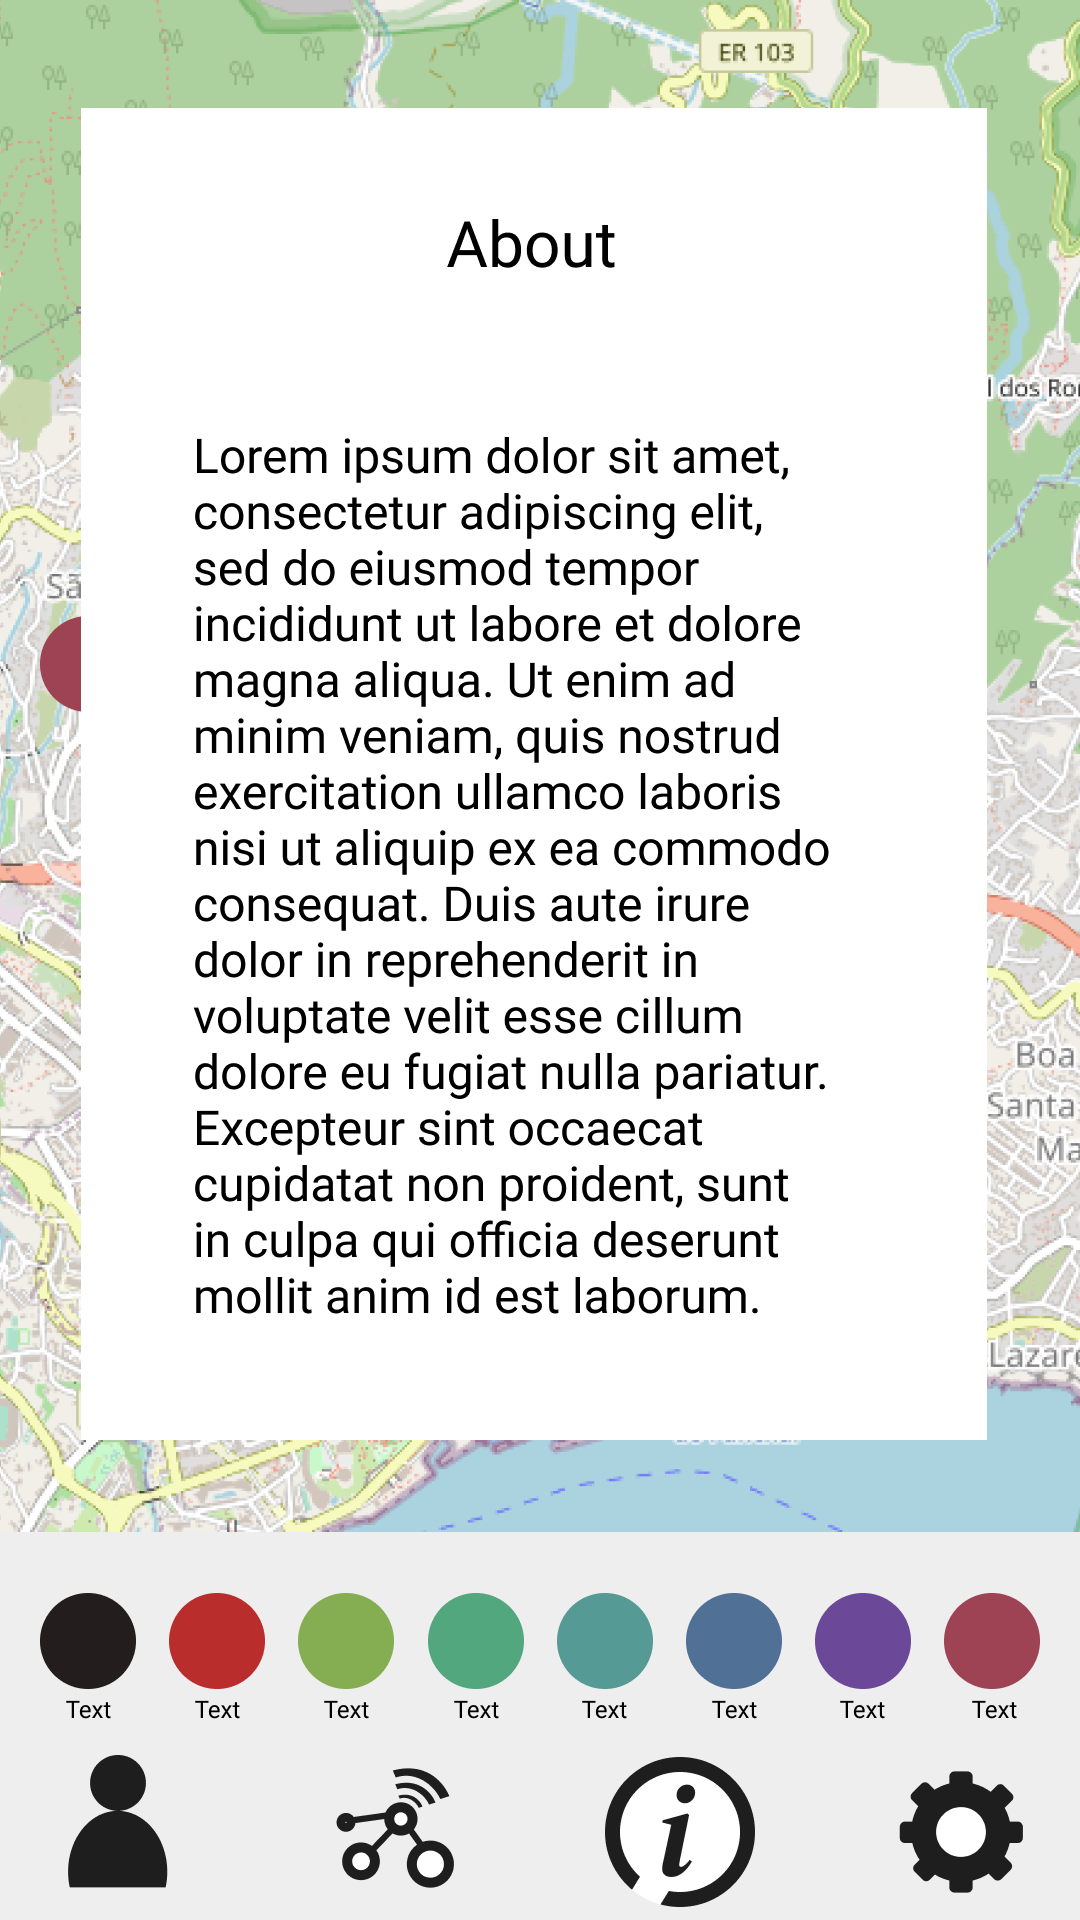
\includegraphics[width=130pt]{../assets/images/low_about.png}
        \caption{}
        \label{fig:about}
    \end{subfigure}%
    \begin{subfigure}{0.33\textwidth}
        \centering
        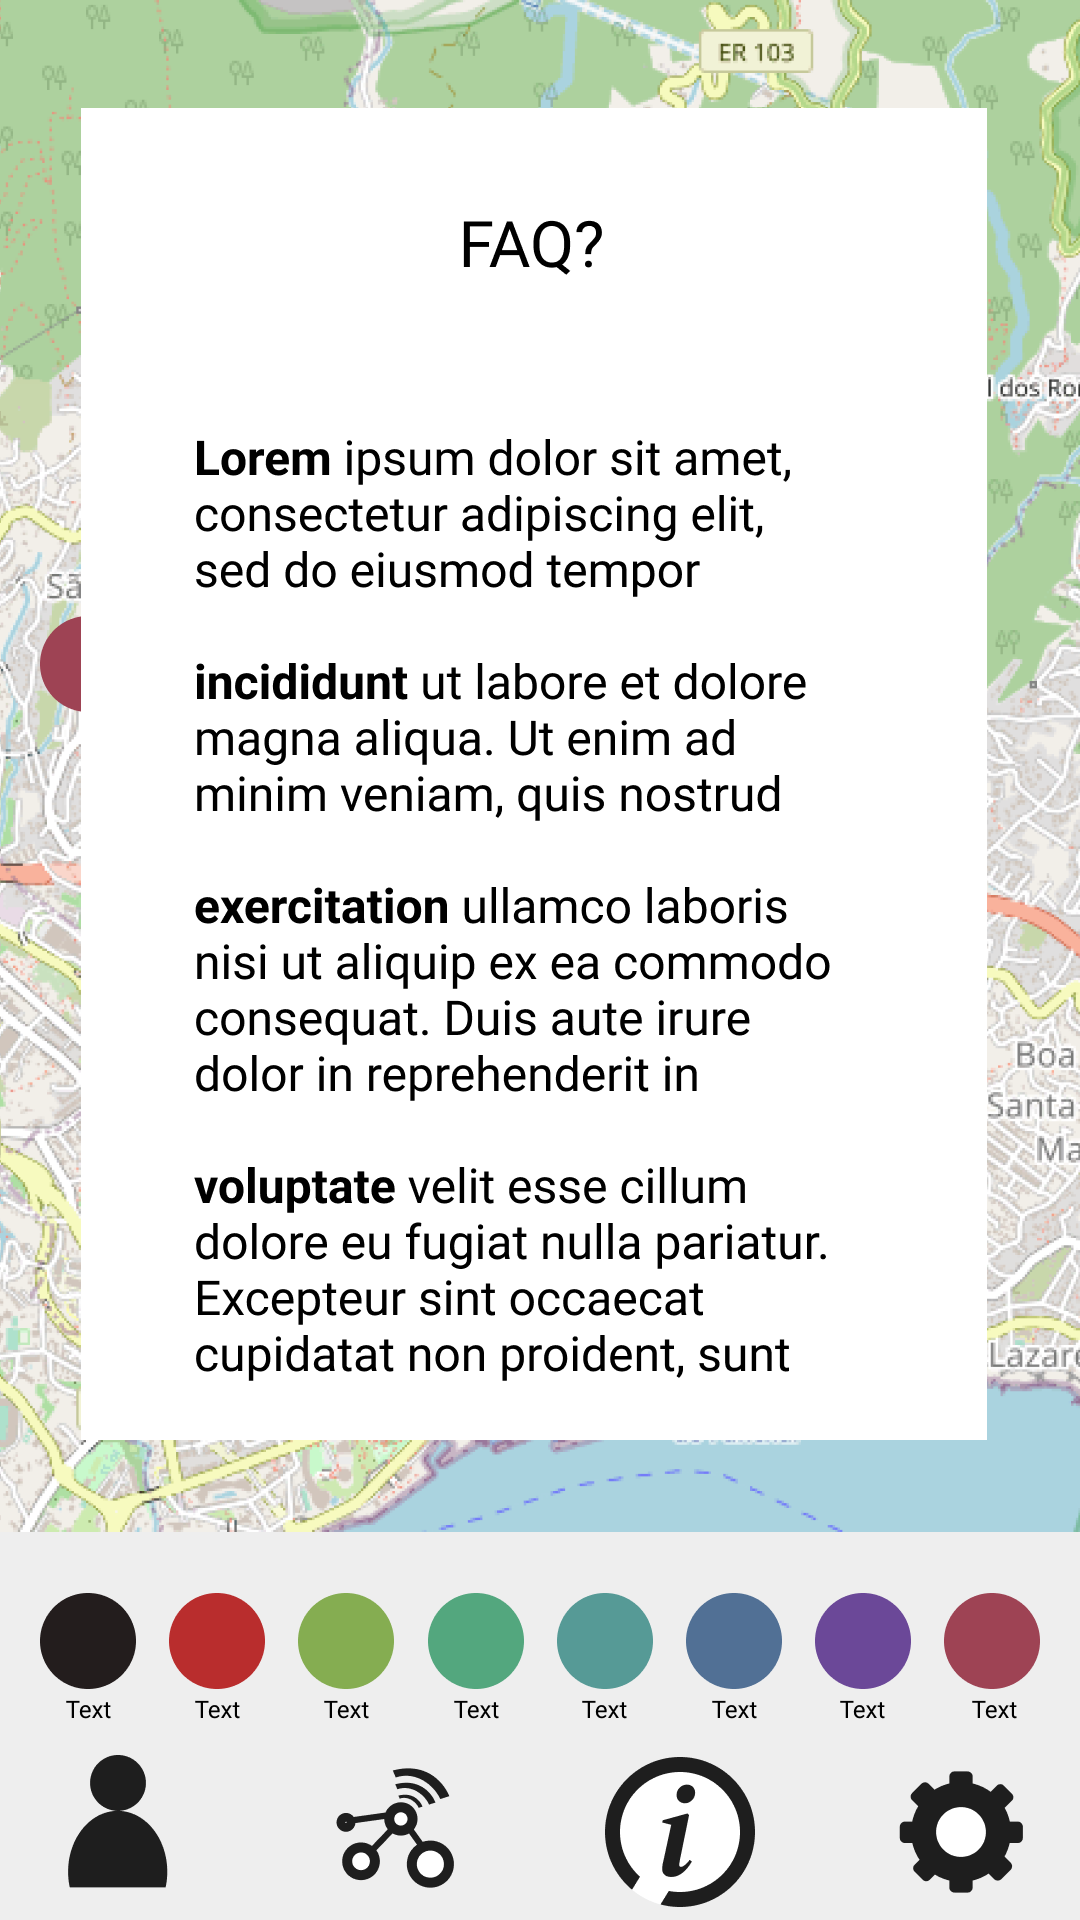
\includegraphics[width=130pt]{../assets/images/low_more_info.png}
        \caption{}
        \label{fig:faq}
    \end{subfigure}%
    \caption{High level prototype of (a) homepage, (b) about and (c) FAQ pages.}
    \label{fig:highlevelprototype}
\end{figure}

Usability tests were conducted in person with X participants of different
ages, professional fields and qualifications. Before doing the tests,
some questions were made to gather the general level of digital literacy
related to IoT and privacy, then the participants were asked to fill in the
survey, if they had not yet done, as this gives some insight into what the
application is about. The usability tests consists of single ease questions
and system usability scale, as can be seen on appendix \ref{appendix:usability_tests}.
The single ease question was used after the participant performed eached task, the
participant would answer how diffucult they though the task was in a
scale of 1 to 7. The system usability scale was used after the participants
performed all tasks, using this system a score of X was achieved.

\section{Challenges}

One of the most difficult points to accomplish in this thesis was the
questionnaire, not the fact of constructing the questionnaire but of
getting participants. Besides being difficult in itself to get a relatively
high number of participants of participants (a few hundred at least)
to be able to draw conclusions with any high degree of confidence, it was
difficult to get to get the potential participants interested in the topic
at hand, because although it seems that many people value their privacy very
highly and think they should protect it in practice they are not very
interested. This may even be because many people do not have much knowledge
about the Internet of Things, and thus feel that they cannot answer the
questionnaire because it is out of their field of knowledge, another
reason may be that the questionnaire seems a little long, because it
takes on average 15 to 20 minutes to answer, and despite being a topic
of interest the time investment in the questionnaire may be considered
too high. Another point to take into consideration regarding the low
number of participants is the way the questionnaire is written and how
it was advertised, i.e., a very formal or technical language may have
been used both in the construction of the questionnaire and in its
dissemination, and the fact that this is a very niche topic may have
"scared" possible participants. However, it should be noted that also
in the literature that has been carried out there is not a great focus
on conducting questionnaires and the ones that have been conducted have
not only focused on the Internet of Things and also have some monetary
incentive for the participants.

% Um dos pontos mais difíceis de realizar nesta tese foi o questionário,
% não o facto de construir o questionário mas sim de angariar participantes.
% Para além de ser difícil por si só conseguir ter um número de participantes
% relativamente alto (algumas centenas, 500 a 1000) para conseguirmos tirar
% conclusões com algum grau de confiança elevado, foi difícil de conseguir
% com que os possíveis participantes se interessassem no tópico em questão,
% pois apesar de parecer que muitas pessoas valorizem muito a sua privacidade
% e achem que devem a proteger na prática não se interessam muito. Isto até
% pode ser porque muitas pessoas não tenham muito conhecimento a nível da
% Internet of Things, e assim acharem que não conseguem responder ao questionário
% por ser fora do seu campo de conhecimento, outra razão pode o questionário
% parecer um pouco longo, pois demora em média 15 a 20 minutos para responder,
% e apesar de até ser um tópico de interesse o investimento de tempo no
% questionário pode ser considerado muito elevado. Outro ponto a ter em consideração
% em relação ao baixo número de participantes é a forma como o questionário
% está escrito e como este foi divulgado, isto é, pode ter sido usado
% uma linguagem muito formal ou técnica tanto na construção do mesmo como
% também na sua divulgação e juntado ao facto de este ser um tópico muito niche
% pode ter "assustando" possíveis participantes. Contudo é de notar que
% também na literatura que tem vindo a ser realizada não há um grande foco
% na realização de questionários e os que têm sido realizados não têm se
% focado somente na Internet of Things e têm também algum incentivo monetário
% para os participantes.
